%%==================================================================%%
%% Author : Perez Ruiz, Alejandro                                   %%
%% Version: 1.0, 08/02/2011                                         %%
%% Version: 1.1, 17/06/2011                                         %%
%%                                                                  %%
%% Memoria del Proyecto Fin de Carrera                              %%
%%==================================================================%%

\documentclass[a4paper,11pt,oneside]{itsas_pfc}

%%==================================================================%%
%%                     My imported packages                         %%
%%==================================================================%%
\usepackage[latin1]{inputenc}
\usepackage{longtable}
\usepackage{array}
\usepackage{url}
\usepackage{amsfonts}
\usepackage[spanish,activeacute]{babel}

% File with main configuration
\input{config/pfc_options.tex}
% File with some names
\input{config/rename.tex}

%=====================================================================%
%                           Thesis's details                          %
%=====================================================================%
\newcommand{\myname}{Alejandro Ruiz P�rez}  % name of author
\newcommand{\myboss}{Pablo S�nchez Barreiro} % name of supervisor
\newcommand{\thesistitle}{Desarrollo de una L�nea de Productos Software \\ para Automatizaci�n de Hogares \\ usando Clases Parciales de C\#}

\newcommand{\englishtitle}{Development of a Software Product Line \\
						   for Automated Houses using C\# Partial Classes}
												  % work title
\newcommand{\worktype}{Proyecto Fin de Carrera}   % work type
\newcommand{\logo}{images/uc.eps}            % logo file (e.g. for the cover)

%=====================================================================%
%                     Definition of my own commands                   %
%=====================================================================%
\newcommand{\nota}[1]{\color{red}$\ll$#1$\gg$\color{black}}
\newcommand{\imp}[1]{{\small{\sf #1}}}
\newcommand{\stereotype}[1]{$\ll${\small{\sf #1}}$\gg$}
\newcommand{\todo}[1]{\color{red}$\ll$TODO: #1$\gg$\color{black}}

\setcounter{minitocdepth}{1}

\begin{document}

% Cover page
 \input{cover/cover.tex}

% \input{cover/supervisorApproval.tex}

% \input{cover/firstPage.tex}

% reset page numbering
\input{config/begin.tex}

% acknowledgement
% \cdpchapter{Agradecimientos}

A mi madre y mi abuela por haberme apoyado en todas mis decisiones acad�micas y por estar siempre conmigo durante todos estos a�oos.

A mi director Pablo S�nchez por ofrecerme la oportunidad de realizar este proyecto y por guiarme y aconsejarme en todo su desarrollo.

A todos los profesores que desde peque�a han sabido transmitirme sus conocimientos y en especial a los profesores de Ingenier�a Inform�tica de la Universidad de Cantabria.

Al Ministerio de Educaci�n por darme la oportunidad de estudiar la carrera que siempre quise gracias a las becas que me han otorgado.
 % acknowledgements

% Prefacio
% %=============================================================================%
% Author : Alejandro P�rez Ruiz                                               %
% Author : Pablo S�nchez Barreiro                                             %
% Version: 1.0, 30/05/2011                                                    %
% Version: 1.1, 06/05/2011                                                    %
% Master Thesis: Resumen                                                      %
%=============================================================================%



\cdpchapter{
\vspace{-80pt}Resumen}

\vspace{-20pt}
El objetivo de una \emph{l�nea de productos software} es crear una infraestructura a partir de la cual se puedan derivar, tan autom�ticamente como sea posible, productos concretos pertenecientes a una familia de productos software. Una \emph{familia de productos software} es un conjunto de aplicaciones software similares, que por tanto comparten una serie de caracter�sticas comunes, pero que tambi�n presentan variaciones entre ellos.

El software para el control de hogares automatizados es un claro ejemplo de dominio donde un enfoque de l�neas de productos software resulta muy adecuado. Dicho dominio presenta un amplio rango de variaciones debido a los diferentes dispositivos que pueden ser controlados (por ejemplo, ventanas, puertas, luces, etc.) y las funciones que se desea que dichos dispositivos realicen (por ejemplo, simulaci�n de presencia, control inteligente de la energ�a, etc.).

El objetivo de este proyecto es crear una l�nea de productos software para el desarrollo de software para hogares inteligentes de forma que se pueda automatizar el proceso de desarrollo de aplicaciones concretas.  Dicha l�nea de productos software ha sido desarrollada en la plataforma .NET, usando las clases parciales de C\# como principal mecanismo para soportar las diferentes variaciones existentes. La especificaci�n de requisitos que debe cumplir la l�nea de productos est� basada en un caso de estudio industrial proporcionado por Siemens AG.

Las ventajas de alas l�neas de productos software es que se pueden crear productos software concretos, pertenecientes a la familia de productos, de forma autom�tica mediante la simple especificaci�n de las caracter�sticas que se desea incluir en un producto concreto. Se reducen los tiempos de desarrollo y en consecuencia el coste asociado a cada producto concreto.

Como resultado del proyecto, se han desarrollado una serie de extensiones para  Visual Studio 2010. Dichos extensiones permiten modelar hogares autom�ticos y/o inteligentes seleccionando las caracter�sticas que mejor se adapten las necesidades del cliente. A continuaci�n, mediante generaci�n de c�digo, se obtiene autom�ticamente el producto deseado.

\paragraph{Palabras Clave} \ \\

L�nea de Productos Software, Desarrollo Software Orientado a Caracter�sticas, TENTE, Clases Parciales C\#, .NET

   % preface

% Preface
% %=============================================================================%
% Author : Alejandro P�rez Ruiz                                               %
% Author : Pablo S�nchez Barreiro                                             %
% Version: 1.0, 30/05/2011                                                    %
% Version: 1.1, 06/06/2011                                                    %
% Master Thesis: Resumen                                                      %
%=============================================================================%

\cdpchapter{Preface}

The goal of a software product line~\cite{pohl:2005} is to create an adequate infrastructure from which specific products within a software products family
can be constructed as automatically as possible. A \emph{family of software products} is a set of similar software applications, which share some common characteristics, but they also present variations between them.

The software to control a smart home is an typical domain where a software product line approach is particularly suitable. This domain provides a wide range of variations due to the different devices to be controlled in each specific software setup (e.g., windows, doors, lights, heaters, etc.) and the functions these devices must execute (e.g., presence simulation, automatic light control, smart energy control, etc.).

This project aims to construct a software product line for automated houses. The final goal is to automate the development process of specific applications belonging to this family of products. This software product line has been developed on the platform .NET. C\# Partial classes have been used as the main mechanism for modularization, composition and management of the different variable features we have found inside this family of software products. The requirements specification for our software product line is based on an industrial case study provided by Siemens AG.

The main benefit of creating such a software product line is to be able to create specific software products automatically by means of simply specifying which features must be included in each software product. This reduces the software development effort, decreasing the cost of each specific product.

This project has produced as a result several extensions to Visual Studio 2010. These plugins allow developers to visually specify which features must be included in a specific product. Then, all the code required for running such a product is automatically obtained using automatic code generation. 

\paragraph{Keywords} \ \\

Software product Lines, Feature-Oriented Software Development, TENTE, C\# Partial Classes, .NET
   % preface

% Toc
% \input{config/toc.tex}

\input{Config/headers.tex}

\input{config/chapters.tex}

% Cap�tulo 1: Introducci�n
% %%==================================================================%%
%% Author : Abascal Fern�ndez, Patricia                             %%
%%          S�nchez Barreiro, Pablo                                 %%
%% Version: 2.1, 14/06/2013                                         %%                                                                                    %%                                                                  %%
%% Memoria del Proyecto Fin de Carrera                              %%
%% Archivo ra�z                                                     %%
%%==================================================================%%

\chapterheader{Introducci�n}{Introducci�n}
\label{chap:introduction}

Este cap�tulo sirve de introducci�n a la presente Memoria de Proyecto Fin de Carrera. Para ello, en primer lugar se describe el contexto general donde se enmarca dicho proyecto y que da lugar al mismo. Se describe luego, a grandes rasgos, el proyecto para la metodolog�a Te.Net, proyecto general de amplio alcance donde se inscribe el presente proyecto. A continuaci�n, se exponen los objetivos principales del proyecto. Por �ltimo, se describe c�mo se estructura el presente documento.

\chaptertoc

\section{Contexto del Proyecto}
\label{sec:intr:introduction}

\input{introduction/theIntroduction.tex}

\section{La metodolog�a Te.NET}
\label{sec:intr:tenet}

%%==================================================================%%
%% Author : Abascal Fern�ndez, Patricia                             %%
%%          S�nchez Barreiro, Pablo                                 %%
%% Version: 1.3, 18/06/2013                                         %%                                                                                    %%                                                                  %%
%% Memoria del Proyecto Fin de Carrera                              %%
%% Introduccion/Metodologia TeNet                                   %%
%%==================================================================%%

Tal como se ha comentado en la secci�n anterior, la metodolog�a Te.Net se trata de una variante de la tecnolog�a TENTE. A diferencia de TENTE, la cual obliga a utilizar como lenguaje de programaci�n final un lenguaje orientado a caracter�sticas que soporte el concepto de \emph{familia de clases}, al estilo de \emph{CaesarJ}~\cite{ivica:2006} u \emph{ObjectTeams}~\cite{stephan:2002}, Te.NEt utiliza como lenguaje de programaci�n destino un lenguaje convencional orientado a objetos, m�s concretamente C\#.

El primer paso a realizar para llevar a cabo este redise�o de la metodolog�a TENTE era analizar c�mo se pod�a dar soporte a la orientaci�n a aspectos en un lenguaje de programaci�n orientado a objetos como C\#. Tras realizar una buscar opciones en el estado del arte actual, se encontr� un prometedor trabajo~\cite{perez:2011} en el cual se propon�a la utilizaci�n de las clases parciales de C\# como mecanismos para dar soporte a la orientaci�n caracter�sticas.

%%==================================================================%%
%% NOTA(Pablo): Esto se pasar�a a la parte de antecedentes           %%
%%==================================================================%%
%%
%% Las \emph{clases parciales} permiten a los desarrolladores fragmentar %% la implementaci�n de una clase en un conjunto de ficheros, cada uno
%% de los cuales contiene una porci�n, o incremento, de una
%% funcionalidad de la clase. Sin embargo, no ofrecen ning�n mecanismo
%% para agrupar o encapsular caracter�sticas, por lo que no es posible
%% ocultar clases y m�todos que pertenecen a una caracter�stica
%% espec�fica de aquellas clases y m�todos que pertenecen a
%% caracter�sticas independientes. Adem�s, permiten a�adir nuevos
%% atributos y m�todos a existentes clases parciales pero no permite
%% sobreescribir o extender m�todos ya existentes.
%%
%%==================================================================%%

Por tanto, se decidi� evaluar dicho trabajo en profundidad con objeto de verificar las ideas propuestas en el mismo. Los experimentos realizados~\cite{sanchez:2010} revelaron diferentes debilidades de las clases parciales como mecanismo para la implementaci�n de l�neas de productos software.

Para solventar los problemas detectados, se cre�, como resultado de otro Proyecto Fin de Carrera presentado en esta misma Facultad, un patr�n de dise�o denominado \emph{Slicer Pattern}~\cite{perez:2011}. Dentro de dicho Proyecto Fin de Carrera se implement� una l�nea de productos software para el desarrollo de software de gesti�n de hogares inteligentes.

Una vez que se hab�a solventado el problema de c�mo soportar la orientaci�n a caracter�sticas en C\#, la siguiente tarea a realizar era la de adaptar los generadores de c�digos originales para que soportasen la generaci�n de c�digo en C\# en lugar de CaesarJ. Esta tarea constituye el objetivo principal de este proyecto, el cual se detalla en la siguiente secci�n.




\section{Motivaci�n y Objetivos}
\label{sec:intr:objetivos}

%%==================================================================%%
%% Author : Abascal Fern�ndez, Patricia                             %%
%%          S�nchez Barreiro, Pablo                                 %%
%% Version: 1.2, 11/06/2013                                         %%                                                                                    %%                                                                  %%
%% Memoria del Proyecto Fin de Carrera                              %%
%% Introduccion/Metodologia TeNet                                   %%
%%==================================================================%%

%%==================================================================%%
%% NOTA(Pablo): Te dejo tres p�rrafos, la idea es que los refundas  %%
%%              en uno y lo ligues con la secci�n anterior. Te      %%
%%              puedes extender un poco en detallar cada objetivo   %%
%%              si lo crees necesario, tal y como hizo Alejandro    %% 
%%==================================================================%%

El principal objetivo de este Proyecto de Fin de Carrera es implementar un conjunto de generadores de c�digo que permitan transformar modelos UML orientados a caracter�sticas en c�digo C\#. Para dar soporte a la orientaci�n a caracter�sticas a nivel de c�digo C\#, se utilizar� el patr�n de dise�o
\emph{Slicer}. Dicho patr�n fue espec�ficamente para tal prop�sito como parte de otro Proyecto Fin de Carrera presentado en esta misma Facultad~\cite{}.

%%%%%%%%%%%% Retoma el objetivo del proyecto %%%%%%%%%%%%
El objetivo de este Proyecto Fin de Carrera es implementar generadores de c�digo que abordar�n tanto la implementaci�n de la familia de productos software cubierta por la l�nea de productos, como la configuraci�n de productos concretos pertenecientes a dicha familia utilizando las prestaciones de las clases parciales en C\# y el Patr�n Slicer. Con esto esperamos haber aclarado el primer p�rrafo de esta secci�n al lector no familiarizado con las l�neas de productos software, clases parciales en lenguaje C\# y/o el Patr�n Slicer.


Tal como se ha descrito al inicio de este apartado, el objetivo del presente Proyecto Fin de Carrera consiste en el desarrollo e implementaci�n de unos generadores de c�digo que permitan la tranformaci�n del dise�o de los modelos en una implementaci�n en c�digo C\# de dichos dise�os, para ello se usar�n las prestaciones que ofrecen el uso de las clases parciales del lenguaje C\# basadas en el patr�n Slicer.


\section{Estructura del Documento}
\label{sec:intr:estructura}

%%==================================================================%%
%% Author : Abascal Fernández, Patricia                             %%
%%          Sánchez Barreiro, Pablo                                 %%
%% Version: 1.3, 18/06/2013                                         %%                                                                                    %%                                                                  %%
%% Memoria del Proyecto Fin de Carrera                              %%
%% Introducción/Roadmap                                             %%
%%==================================================================%%

\todo{COMPLETAR}

Tras este capítulo introductorio, el resto del documento se estructura como sigue: el
Capítulo 2 describe brevemente los conceptos necesarios, tales como ------------ para poder entender la presente memoria. El Capítulo 3 explica -------- fases seguidas para la realización del proyecto, así como
los aspectos generales del mismo. El Capítulo 4 describe el desarrollo de la infraestructura
necesaria para la derivación de productos concretos, mientras que el Capítulo 5 describe como
se derivan dichos productos concretos de forma automática desde dicha infraestructura.
Por último, el Capítulo 6 analiza brevemente las conclusiones extraídas tras la realización
de este proyecto, así como posibles trabajos futuros.




% Cap�tulo 2: Resumen del Estado del Arte
% %=============================================================================%
% Author : Alejandro P�rez Ruiz                                               %
% Author : Pablo S�nchez Barreiro                                             %  % Version: 1.0, 07/03/2011                                                    %
% Master Thesis: Background, master file                                      %
%=============================================================================%

\chapterheader{Antecedentes}{Antecedentes}
\label{chap:introduction}

% Introducci�n al cap�tulo

\chaptertoc

\section{L�neas de Productos Software}

% Explica que es una l�nea de productos software, objetivos y terminolog�a
% \footnote{} 

\section{Programaci�n Orientada a Caracter�sticas}

% Objetivos de la orientaci�n a caracter�sticas

\subsection{Limitaciones de la Orientaci�n a Objetos para la Programaci�n Orientada a Caracter�sticas}

% Limitaciones de los lenguajes OO para FOP
% - Cuentas el ejemplo de las expresiones
% - Muestras la soluci�n en C#.
% - Resumes los problemas

\subsection{Ventajas de los lenguajes orientados a caracter�sticas}

% P�rrafo introducci�n
% Introducci�n CaesarJ 
% Ejemplo en CeasrJ, resaltando ventajas

\section{Clases Parciales C#}

% Qu� hace esto aqu�

% Explicar que son brevemente, y ejemplo usando las expresiones

\section{Caso de Estudio: Hogares \emph{Inteligentes} Automatizados}

% Resumir lo que aparece en diversos documentos



% Cap�tulo 3: Definici�n y Planificaci�n del Proyecto

% %%==================================================================%%
%% Author : Abascal Fern�ndez, Patricia                             %%
%%          S�nchez Barreiro, Pablo                                 %%
%% Version: 1.2, 18/06/2013                                         %%
%%                                                                  %%
%% Memoria del Proyecto Fin de Carrera                              %%
%% Background/Generaci�n de C�digo con Epsilon                      %%
%===================================================================%%

Como se ha comentado con anterioridad, el objetivo de este Proyecto Fin de Carrera es el desarrollo de una serie de generadores de c�digo que permitan automatizar la aplicaci�n del \emph{Slicer Pattern}. Dichos generadores de c�digo se desarrollar�n utilizando un moderno enfoque de \emph{Ingenier�a de L�neas de Productos Software}. Por tanto, el proceso de desarrollo del presente proyecto queda pr�cticamente determinado por dicho enfoque, el cual posee un proceso de desarrollo bien definido, el cual se describi� en la secci�n~\ref{sec:back:spl}. La Figura~\ref{fig:planning} muestra como dicho proceso de desarrollo se ha instanciado para nuestro caso particular.

\begin{figure}[!tb]
    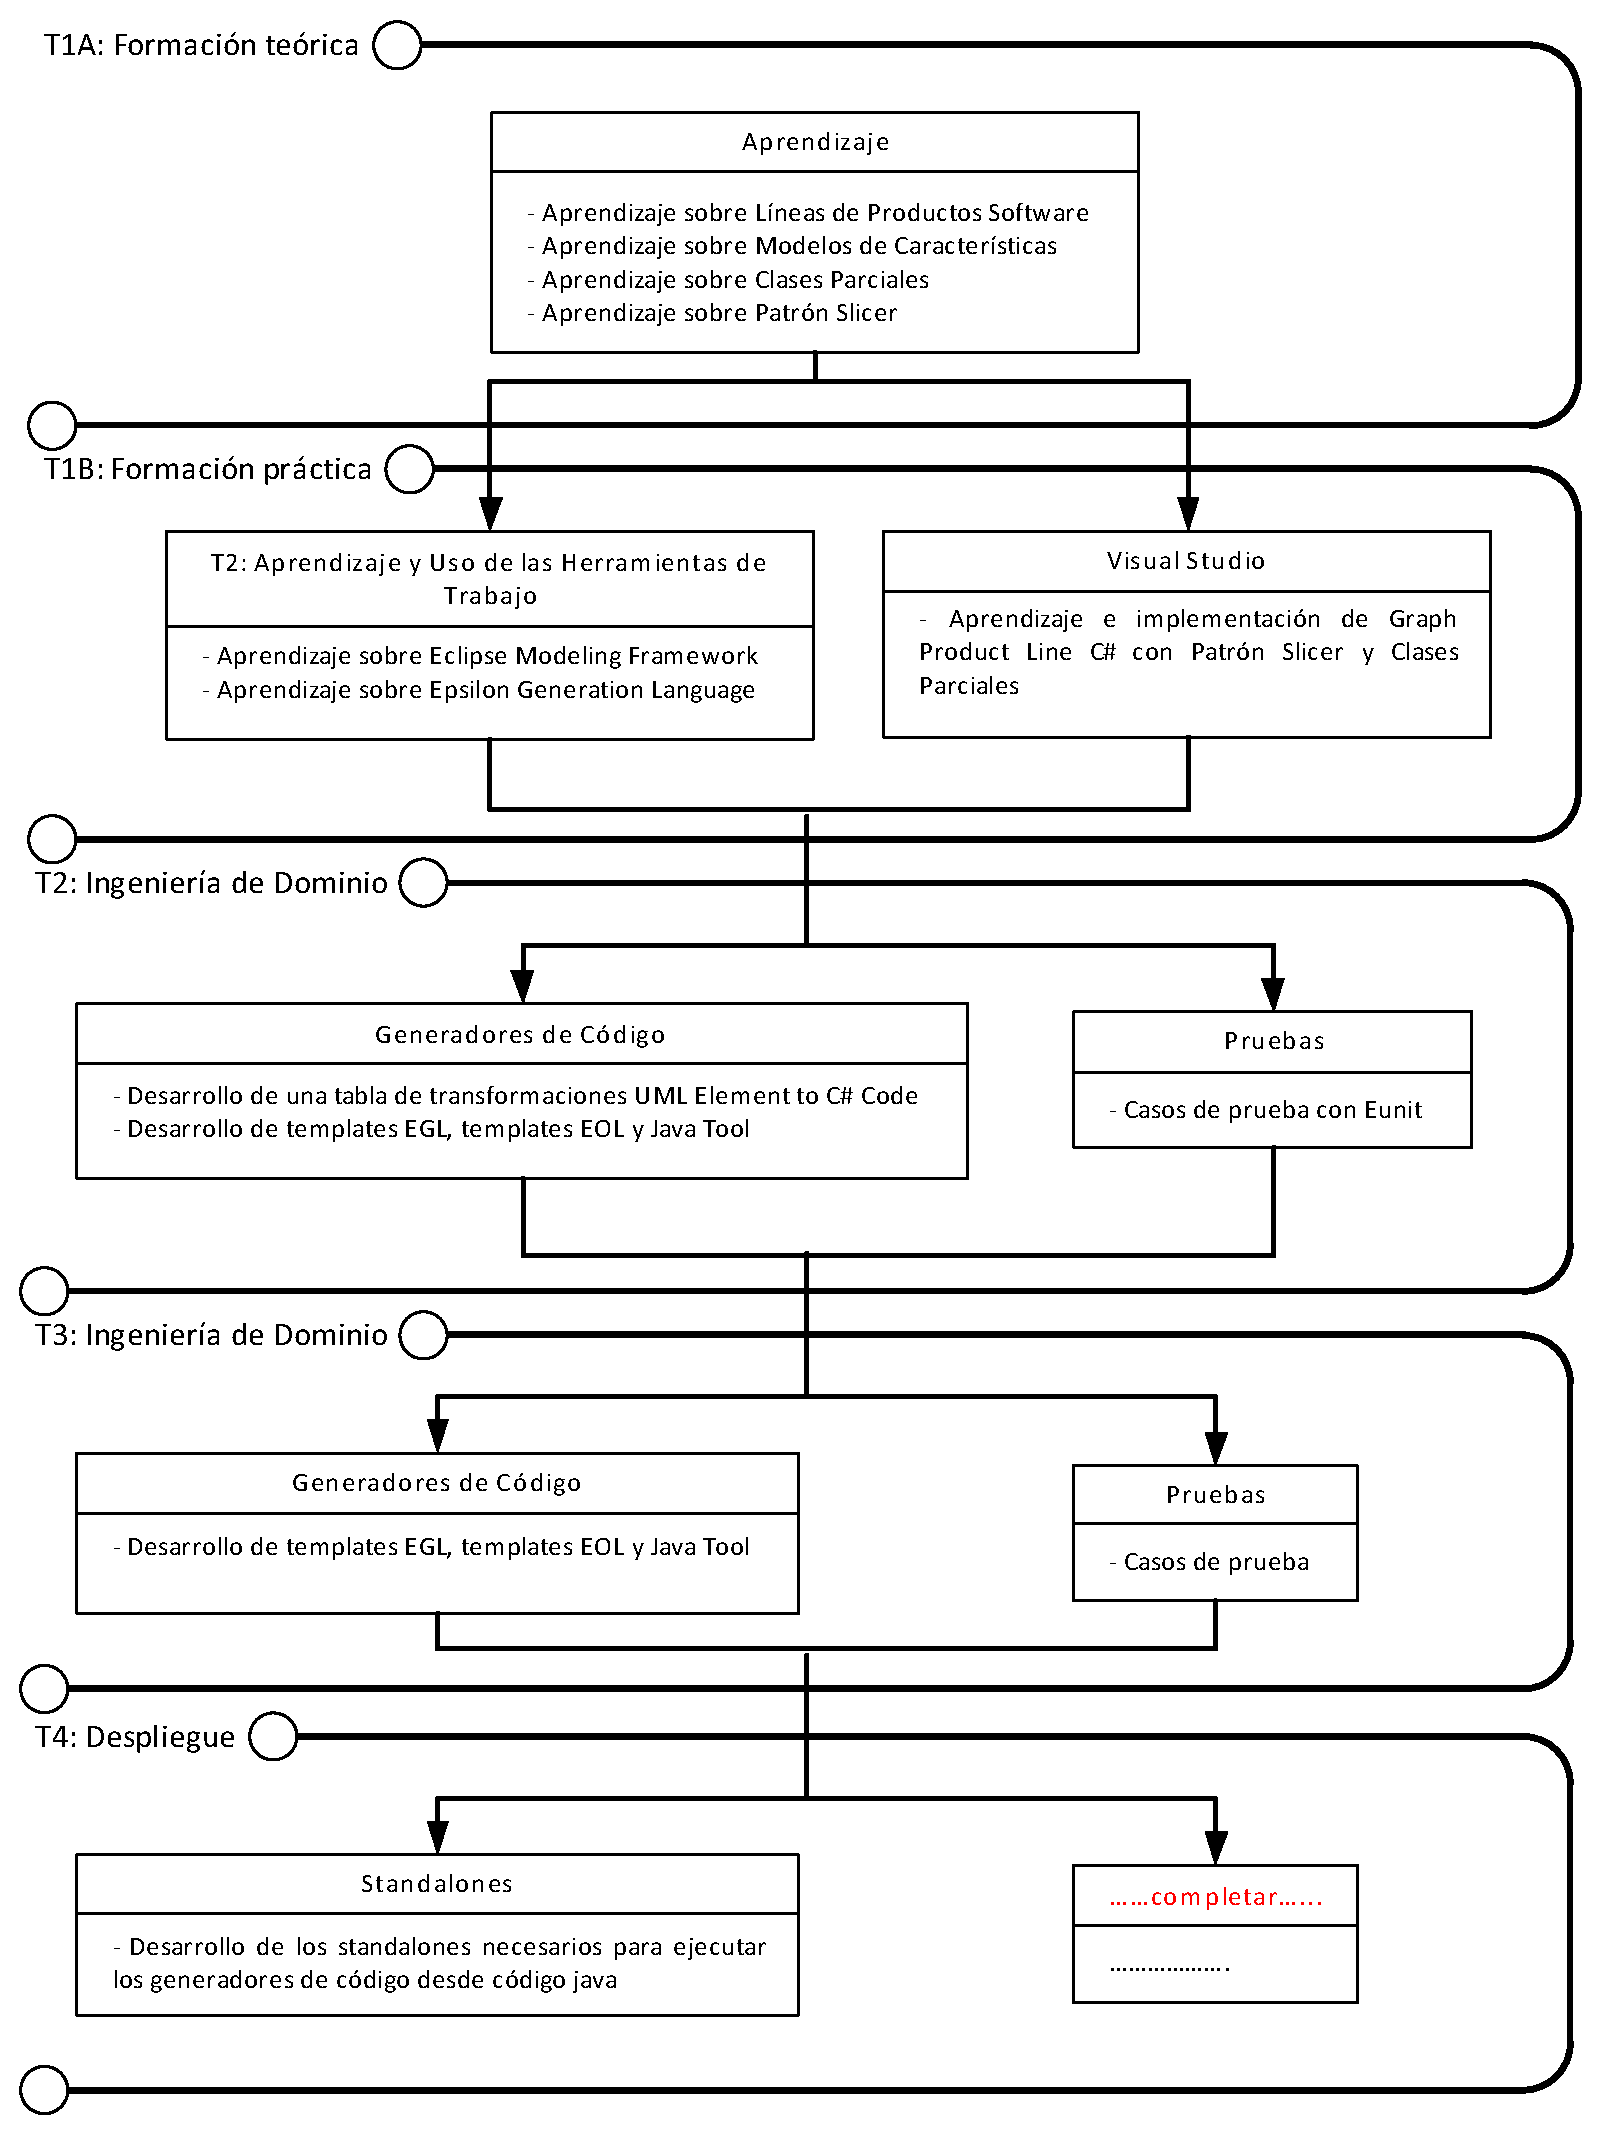
\includegraphics[scale=0.74]{background/images/planning.eps}
    \caption{Proceso de desarrollo del Proyecto Fin de Carrera}
    \label{fig:planning}
\end{figure}

Obviamente, la primera tarea (Figura~\ref{fig:planning}-\emph{T1A} y \emph{T1B}) en este proceso de desarrollo fue la de adquirir los conocimientos necesarios para la realizaci�n de todas las tareas posteriores. Ello implicaba adquirir los conocimientos relacionados con las \emph{L�neas de Producto Software}~\cite{pohl:2010, kakola:2006} en general y con el dise�o orientado a modelos~\cite{kastner:2008}, las clases parciales~\cite{sanchez:2010} y el patr�n slicer ~\cite{perez:2011} en particular.

Dado que el proyecto se deb�a implementar con una herramienta para el desarrollo software dirigido por modelos, denominado \emph{Epsilon}~\cite{kolovos:2008}, el siguiente paso (Figura~\ref{fig:planning}-\emph{T1B} y \emph{T1B}) fue familiarizarse con dicha herramienta y adquirir ciertos conocimientos sobre la utilizaci�n de EMF (\emph{Eclipse Modelling Framework})~\cite{steinberg:2008} para la definici�n de metamodelos y sobre los lenguajes a utilizar para la generaci�n de c�digo, EGL (\emph{Epsilon Generation Language})~\citep{dimitrios:2012} y EOL (\emph{Epsilon Object Language})~\citep{dimitrios:2012}. Adem�s, por exigencias de los usuarios finales de este producto, el c�digo generado deb�a ser editable como un proyecto de Visual Studio 2010, por lo que a continuaci�n se procedi� al manejo y aprendizaje de uso de dicha herramienta mediante la creaci�n de un proyecto de l�nea de productos software aplicando los conceptos te�ricos aprendidos en la etapa \emph{T1A}, es decir las clases parciales C\# y el \emph{Slicer Pattern}.

Tras esta tarea inicial de adquisici�n de conocimientos previos, el resto del proyecto se estructura como un proyecto de Ingenier�a de L�neas de Producto Software. Consecuentemente, la primera tarea tras la fase inicial de documentaci�n (Figura~\ref{fig:planning}-\emph{T2}) fue la fase dedicada a la implementaci�n de la fase de \emph{Ingenier�a del Dominio}, es decir, la implementaci�n de los generadores de c�digo necesarios para transformar el modelo UML dado en un proyecto Visual Studio escrito en lenguaje C\# y que estuviera implementado acorde a las clases parciales C\# y el \emph{Slicer Pattern}, conocimientos adquiridos en la fase \emph{T1} de la planificaci�n. Completando el desarrollo de esta etapa con las pruebas pertinentes mediante el uso de la herramienta EUnit~\citep{dimitrios:2012}.

A continuaci�n, de acuerdo con lo expuesto en la secci�n anterior, procedimos a desarrollar la implementaci�n de la fase de \emph{Ingenier�a de Aplicaci�n} (Figura~\ref{fig:planning}-\emph{T3}) que se desarroll� de manera an�loga a la fase \emph{T2}.

%% %% %% %% %% %% %% %% %% %% %% %% %% %% %% %% %% %% %% %% %% %% %% %% %% %%
\todo{completar con la explicaci�n de la creaci�n del plugin cuando lo termine}
%% %% %% %% %% %% %% %% %% %% %% %% %% %% %% %% %% %% %% %% %% %% %% %% %% %%

En este punto del proceso de desarrollo ten�amos implementado el editor requerido, por lo que s�lo restaba proceder a su despliegue (Figura~\ref{fig:planning}-\emph{T4}). Este despliegue implicaba su integraci�n dentro de la arquitectura de plugins de Eclipse. Tras dicha integraci�n, se procedi� a realizar una serie de pruebas de aceptaci�n, destinadas a comprobar que el trabajo realizado satisfac�a las necesidades de los usuarios finales que iban a utilizar el producto creado.


% Cap�tulo 4: Domain Engineering

% %%==================================================================%%
%% Author : Abascal Fern�ndez, Patricia                             %%
%% Author : S�nchez Barreiro, Pablo                                 %%
%% Version: 1.1, 21/04/2013                                         %%
%%                                                                  %%
%% Memoria del Proyecto Fin de Carrera                              %%
%% Cap�tulo Domain Engineering, Archivo ra�z                        %%
%%==================================================================%%

\chapterheader{Ingenier�a del Dominio}{Ingenier�a del Dominio}
\label{chap:domain}

Este cap�tulo describe el proceso de desarrollo de los generadores de c�digo para la fase de \emph{Ingenier�a del Dominio} dentro de la metodolog�a Te.Net. Para ello primero describiremos las reglas que especifican c�mo se transforman los elementos del modelo a c�digo C\#. A continuaci�n,  profundizaremos en el desarrollo e implementaci�n de los generadores de c�digo. Para ilustrar c�mo funcionan los generadores de c�digo, proporcionaremos un ejemplo sencillo. Concluiremos detallando c�mo se han realizado las pruebas de los generadores de c�digo creados.

\chaptertoc

\section{Introducci�n}
\label{domain:sec:intro}

%%==================================================================%%
%% Author : Abascal Fern�ndez, Patricia                             %%
%%          S�nchez Barreiro, Pablo                                 %%
%% Version: 2.1, 14/06/2013                                         %%                                                                                    %%                                                                  %%
%% Memoria del Proyecto Fin de Carrera                              %%
%% Archivo ra�z                                                     %%
%%==================================================================%%

\chapterheader{Introducci�n}{Introducci�n}
\label{chap:introduction}

Este cap�tulo sirve de introducci�n a la presente Memoria de Proyecto Fin de Carrera. Para ello, en primer lugar se describe el contexto general donde se enmarca dicho proyecto y que da lugar al mismo. Se describe luego, a grandes rasgos, el proyecto para la metodolog�a Te.Net, proyecto general de amplio alcance donde se inscribe el presente proyecto. A continuaci�n, se exponen los objetivos principales del proyecto. Por �ltimo, se describe c�mo se estructura el presente documento.

\chaptertoc

\section{Contexto del Proyecto}
\label{sec:intr:introduction}

\input{introduction/theIntroduction.tex}

\section{La metodolog�a Te.NET}
\label{sec:intr:tenet}

%%==================================================================%%
%% Author : Abascal Fern�ndez, Patricia                             %%
%%          S�nchez Barreiro, Pablo                                 %%
%% Version: 1.3, 18/06/2013                                         %%                                                                                    %%                                                                  %%
%% Memoria del Proyecto Fin de Carrera                              %%
%% Introduccion/Metodologia TeNet                                   %%
%%==================================================================%%

Tal como se ha comentado en la secci�n anterior, la metodolog�a Te.Net se trata de una variante de la tecnolog�a TENTE. A diferencia de TENTE, la cual obliga a utilizar como lenguaje de programaci�n final un lenguaje orientado a caracter�sticas que soporte el concepto de \emph{familia de clases}, al estilo de \emph{CaesarJ}~\cite{ivica:2006} u \emph{ObjectTeams}~\cite{stephan:2002}, Te.NEt utiliza como lenguaje de programaci�n destino un lenguaje convencional orientado a objetos, m�s concretamente C\#.

El primer paso a realizar para llevar a cabo este redise�o de la metodolog�a TENTE era analizar c�mo se pod�a dar soporte a la orientaci�n a aspectos en un lenguaje de programaci�n orientado a objetos como C\#. Tras realizar una buscar opciones en el estado del arte actual, se encontr� un prometedor trabajo~\cite{perez:2011} en el cual se propon�a la utilizaci�n de las clases parciales de C\# como mecanismos para dar soporte a la orientaci�n caracter�sticas.

%%==================================================================%%
%% NOTA(Pablo): Esto se pasar�a a la parte de antecedentes           %%
%%==================================================================%%
%%
%% Las \emph{clases parciales} permiten a los desarrolladores fragmentar %% la implementaci�n de una clase en un conjunto de ficheros, cada uno
%% de los cuales contiene una porci�n, o incremento, de una
%% funcionalidad de la clase. Sin embargo, no ofrecen ning�n mecanismo
%% para agrupar o encapsular caracter�sticas, por lo que no es posible
%% ocultar clases y m�todos que pertenecen a una caracter�stica
%% espec�fica de aquellas clases y m�todos que pertenecen a
%% caracter�sticas independientes. Adem�s, permiten a�adir nuevos
%% atributos y m�todos a existentes clases parciales pero no permite
%% sobreescribir o extender m�todos ya existentes.
%%
%%==================================================================%%

Por tanto, se decidi� evaluar dicho trabajo en profundidad con objeto de verificar las ideas propuestas en el mismo. Los experimentos realizados~\cite{sanchez:2010} revelaron diferentes debilidades de las clases parciales como mecanismo para la implementaci�n de l�neas de productos software.

Para solventar los problemas detectados, se cre�, como resultado de otro Proyecto Fin de Carrera presentado en esta misma Facultad, un patr�n de dise�o denominado \emph{Slicer Pattern}~\cite{perez:2011}. Dentro de dicho Proyecto Fin de Carrera se implement� una l�nea de productos software para el desarrollo de software de gesti�n de hogares inteligentes.

Una vez que se hab�a solventado el problema de c�mo soportar la orientaci�n a caracter�sticas en C\#, la siguiente tarea a realizar era la de adaptar los generadores de c�digos originales para que soportasen la generaci�n de c�digo en C\# en lugar de CaesarJ. Esta tarea constituye el objetivo principal de este proyecto, el cual se detalla en la siguiente secci�n.




\section{Motivaci�n y Objetivos}
\label{sec:intr:objetivos}

%%==================================================================%%
%% Author : Abascal Fern�ndez, Patricia                             %%
%%          S�nchez Barreiro, Pablo                                 %%
%% Version: 1.2, 11/06/2013                                         %%                                                                                    %%                                                                  %%
%% Memoria del Proyecto Fin de Carrera                              %%
%% Introduccion/Metodologia TeNet                                   %%
%%==================================================================%%

%%==================================================================%%
%% NOTA(Pablo): Te dejo tres p�rrafos, la idea es que los refundas  %%
%%              en uno y lo ligues con la secci�n anterior. Te      %%
%%              puedes extender un poco en detallar cada objetivo   %%
%%              si lo crees necesario, tal y como hizo Alejandro    %% 
%%==================================================================%%

El principal objetivo de este Proyecto de Fin de Carrera es implementar un conjunto de generadores de c�digo que permitan transformar modelos UML orientados a caracter�sticas en c�digo C\#. Para dar soporte a la orientaci�n a caracter�sticas a nivel de c�digo C\#, se utilizar� el patr�n de dise�o
\emph{Slicer}. Dicho patr�n fue espec�ficamente para tal prop�sito como parte de otro Proyecto Fin de Carrera presentado en esta misma Facultad~\cite{}.

%%%%%%%%%%%% Retoma el objetivo del proyecto %%%%%%%%%%%%
El objetivo de este Proyecto Fin de Carrera es implementar generadores de c�digo que abordar�n tanto la implementaci�n de la familia de productos software cubierta por la l�nea de productos, como la configuraci�n de productos concretos pertenecientes a dicha familia utilizando las prestaciones de las clases parciales en C\# y el Patr�n Slicer. Con esto esperamos haber aclarado el primer p�rrafo de esta secci�n al lector no familiarizado con las l�neas de productos software, clases parciales en lenguaje C\# y/o el Patr�n Slicer.


Tal como se ha descrito al inicio de este apartado, el objetivo del presente Proyecto Fin de Carrera consiste en el desarrollo e implementaci�n de unos generadores de c�digo que permitan la tranformaci�n del dise�o de los modelos en una implementaci�n en c�digo C\# de dichos dise�os, para ello se usar�n las prestaciones que ofrecen el uso de las clases parciales del lenguaje C\# basadas en el patr�n Slicer.


\section{Estructura del Documento}
\label{sec:intr:estructura}

%%==================================================================%%
%% Author : Abascal Fernández, Patricia                             %%
%%          Sánchez Barreiro, Pablo                                 %%
%% Version: 1.3, 18/06/2013                                         %%                                                                                    %%                                                                  %%
%% Memoria del Proyecto Fin de Carrera                              %%
%% Introducción/Roadmap                                             %%
%%==================================================================%%

\todo{COMPLETAR}

Tras este capítulo introductorio, el resto del documento se estructura como sigue: el
Capítulo 2 describe brevemente los conceptos necesarios, tales como ------------ para poder entender la presente memoria. El Capítulo 3 explica -------- fases seguidas para la realización del proyecto, así como
los aspectos generales del mismo. El Capítulo 4 describe el desarrollo de la infraestructura
necesaria para la derivación de productos concretos, mientras que el Capítulo 5 describe como
se derivan dichos productos concretos de forma automática desde dicha infraestructura.
Por último, el Capítulo 6 analiza brevemente las conclusiones extraídas tras la realización
de este proyecto, así como posibles trabajos futuros.




\section{Transformaciones de Modelo UML a C\#}
\label{domain:sec:transf}

%%==================================================================%%
%% Author : Abascal Fern�ndez, Patricia                             %%
%% Author : S�nchez Barreiro, Pablo                                 %%
%% Version: 1.4, 29/04/2013                                         %%
%%                                                                  %%
%% Memoria del Proyecto Fin de Carrera                              %%
%% Domain Engineering/Transformaci�n UML a C#                       %%
%%==================================================================%%



 \begin{figure}[!tb]
  \centering
  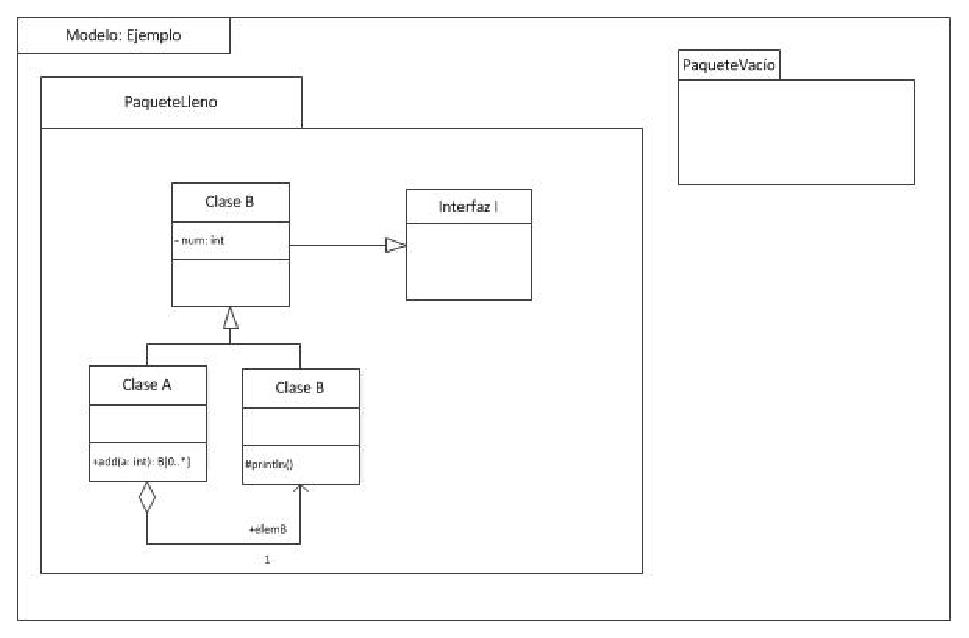
\includegraphics[width=.75\linewidth]{domainEngineering/images/Transformaciones.eps} \\
  \caption{Ejemplo de Modelo UML simplificado}
  \label{dom:fig:ejemplo}
\end{figure}


Como hemos comentado, el primer paso para desarrollar una transformaci�n de modelo a c�digo es: (1) identificar los distintos casos o tipos de entrada con los que nos podemos encontrar; y (2) hallar un equivalente en el lenguaje destino (C\# en nuestro caso). A continuaci�n, mostramos los casos identificados (c�mo t�tulo de cada subsecci�n), y por cada caso, comentamos las equivalencias propuestas. Ciertas de estas reglas son espec�ficas para l�neas de productos software, mientras que otras, como la transformaci�n de las asociaciones, son aplicables a cualquier transformaci�n de UML 2.0 a C#.
Cada regla de transformaci�n la ilustramos utilizando el ejemplo de la Figura~\ref{back:fig:smartHome}.

\subsection{Modelo}

Un modelo UML, es decir, el elemento ra�z que contiene al resto de los elementos de un modelo UML, se transforma en el \emph{namespace} para el proyecto C\#. Los \emph{namespaces} permiten agrupar entidades tales como paquetes, clases, objetos y funciones bajo el mismo nombre. De esta forma, se pueden tener varios \emph{namespaces} en el mismo proyecto que son independientes entre s�.

Recordar que para que varias clases parciales puedan ser combinadas, �stas deben pertenecer a un mismo \emph{namespace}. Por tanto, se utiliza como nombre de dicho \emph{namespace}, el nombre del modelo UML 2.0 que sirve de entrada a los generadores de c�digo.

Adem�s, al transformar el modelo UML 2.0, se crea un proyecto Visual Studio 2010, inicialmente vac�o, con el mismo nombre que el modelo UML 2.0.

Para el caso de la Figura~\ref{back:fig:smartHome}, el nombre del modelo, el cual no aparece en el diagrama, es \emph{SmartHome}. Por tanto, se crear�a un proyecto Visual Studio 2010, con \emph{SmartHome} como nombre. Dentro de dicho proyecto, se crear�a un \emph{namespace} denominado \emph{SmartHome}.

\subsection{Paquete}

Cada paquete UML 2.0 representa en nuestro caso una familia de clases, la cual encapsula una caracter�stica. Por tanto, por cada paquete UML 2.0, se crea una nueva carpeta o directorio, con el mismo nombre que el paquete, en el proyecto Visual Studio 2010 creado al transformar el modelo que contiene dicho paquete. En dicho directorio se colocar�n todos los ficheros resultantes de transformar el contenido de dicho paquete.

Por ejemplo, para el caso de la Figura~\ref{back:fig:smartHome}, durante la transformaci�n del paquete \imp{WindowMng}, se crear�a una nueva carpeta dentro del proyecto Visual Studio 2010 generado, denominada \imp{WindowMng}. Lo mismo se aplicar�a al resto de los paquetes.

\subsection{Tipos primitivos}
\label{subsec:domain:primitiveType}

Por cada tipo primitivo de UML 2.0, se establece una correspondencia con los tipos primitivos de C\#. Por ejemplo, un \emph{String} de UML 2.0 se transforma en \emph{String} de C\#. Un \emph{boolean} de UML 2.0 se transforma en un \emph{bool} de C\#. Esta correspondencia es bastante directa y no presenta problemas m�s de all� de tener que renombrar algunos tipos.

\subsection{Clases Enumeradas}

Cada clase enumerada UML 2.0, se transforma en un enumerado de C\#, con el mismo nombre que el enumerado UML 2.0. A continuaci�n, se procesan los literales de la clase enumerado UML 2.0, a�adiendo un literal con el mismo nombre al enumerado creado en C#.

Por ejemplo, la clase enumerada \imp{TempUnits} de la caracter�stica \imp{HeaterMng} se transformar�a en un enumerado de C\#, con nombre \imp{TempUnits}, perteneciente al \emph{namespace} \imp{HeaterMng}, y con \imp{CELSIUS} y \imp{FARENHEIT} como literales. El Listado~\ref{dom:code:enum} muestra el c�digo resultante de esta transformaci�n.

\begin{lstlisting} [basicstyle=\ttfamily\scriptsize,language=CSharp, captionpos=b,
                    caption=C�digo generado para la clase enumerada \imp{TempUnits},
                    label=dom:code:enum]
01 namespace SmartHome{
02    enum TempUnits {
03        CELSIUS,
04        FARENHEIT
05    };
06 }
\end{lstlisting}

\subsection{Clase}
\label{subsec:domain:class}
Por cada clase UML 2.0 encontrada dentro de un paquete, se genera una clase parcial sita en el directorio correspondiente al paquete al cual pertenece. El nombre de la clase parcial es el mismo que el de la clase UML 2.0.

Por ejemplo, para la clase \emph{WindowCtrl}, del paquete \emph{WindowMng}, se crear�a una clase parcial p�blica, denominada \emph{WindowCtrl}, y sita en la carpeta del proyecto \emph{WindowMng}.

A continuaci�n, se procesan los contenidos de dicha clase, tal como se describe a continuaci�n.

\subsection{Atributo}
\label{subsec:domain:atrib}
Cada atributo de una clase en UML 2.0 se transforma en una propiedad de C\#, perteneciente a clase parcial correspondiente a la clase que posee el atributo en el modelo UML 2.0. Dicha propiedad tendr� siempre visibilidad \emph{protegida} (\emph{protected}), salvo que estuviese declarada como \emph{privada} (\emph{private}) en el modelo UML 2.0, en cuyo caso se mantendr� la visibilidad privada.

Si el atributo era p�blico en el modelo UML, se le generar�n m�todos de acceso (\emph{getter} y \emph{setter}) a dicha propiedad. Si el atributo fuese de solo lectura o derivado, no se le generar�a m�todo de escritura (\emph{setter}).

Si el atributo fuese est�tico (\emph{static}), se generar� como est�tico en el c�digo C\#, y no se le generar�n m�todos de acceso.

Si el tipo del atributo es un tipo primitivo y el atributo no es multivaluado, es decir, la cota superior de su multiplicidad es igual a 1, se utiliza como tipo su correspondiente en C\#, de acuerdo las correspondencias comentadas en la Secci�n~\ref{subsec:domain:primitiveType}. Si el tipo fuese una clase u otro tipo no primitivo, el tipo ser� el nombre resultante de transformar dicho elemento no primitivo.

Por ejemplo, el atributo \imp{id} de la clase \imp{Actuator}, dentro de la caracter�stica \imp{BaseSystem}, se transformar�a en una propiedad llamada \imp{id}, de la clase \imp{Actuator}, sita en la carpeta \imp{BaseSystem}, y perteneciente al \emph{namespace} \imp{SmartHome}. Como tipo para dicha propiedad, se utilizar�a \imp{Int}.

Para el caso del atributo \imp{units} de la clase \imp{Actuator}, dentro de la caracter�stica \imp{HeaterMng}, se utilizar�a como tipo \imp{TempUnits}, ya que ser�a �ste el nombre del enumerado resultante de transformar la clase enumerada que sirve como tipo de este atributo.

Si el atributo fuese un atributo un atributo multivaluado, es decir, la cota superior de su multiplicidad es superior a 1, el tipo de la propiedad generada ser� una colecci�n que use como tipo base el tipo del atributo. Dependiendo de ciertas propiedades del atributo \imp{isOrdered} e \imp{isUnique}, se deber� utilizar un tipo de colecci�n u otro:

%\todo{Explicar el tipo de colecci�n elegida en cada caso y por qu�}
\begin{itemize}
  \item Si el atributo tiene la propiedad \imp{isOrdered=false} e \imp{isUnique=false} estamos ante una colecci�n que admite elementos repetidos y no precisa estar ordenada, por tanto una \imp{ICollection}.
  \item Si el atributo tiene la propiedad \imp{isOrdered=false} e \imp{isUnique=true} se trata de un conjunto \imp{ISet} ya que la colecci�n es de elementos �nicos y no es necesario que est� ordenada.
  \item Si el atributo tiene la propiedad \imp{isOrdered=true} e \imp{isUnique=false} se corresponde con una propiedad de tipo lista \imp{IList} porque son elementos en los que el orden es relevante y admite repeticiones.
  \item En �ltimo lugar, si el atributo tiene la propiedad \imp{isOrdered=true} e \imp{isUnique=true} estamos ante un caso raro y no utilizado del que no se conocen equivalencias en lenguaje C\# por lo que realiza una transformaci�n a \imp{IList}, haciendo saber al usuario final durante el proceso que se ha realizado dicha transformaci�n, en el caso de que fuera necesaria.
\end{itemize}
 
\subsection{Extremos de asociaci�n}
Por cada asociaci�n entre clases en UML 2.0 se transforma en una asociaci�n C\#. Estas asociaciones pueden ser de dos tipos:
\begin{itemize}
  \item Unidireccional. Por ejemplo, la asociaci�n \imp{indoorThem} de la caracter�stica \imp{SmartEnergyMng} indica que la clase \imp{Gateway} de dicha caracter�stica dispone de una propiedad de tipo \imp{ThermometerCtrl} de car�cter monovaluado puesto que presenta multiplicidad 1. Por otro lado, en la asociaci�n \imp{actuators} de la caracter�stica \imp{InitialModel} se aprecia que dicha propiedad es de car�cter multivaluado en tal caso se proceder�a a analizar el tipo de colecci�n de la que se trata tal como se describi� en la Secci�n \ref\label{subsec:domain:atrib}.
  \item Bidireccional. Aquellos casos en los que la asociaci�n tiene lugar en ambos sentidos y por tanto las dos clases involucradas poseen atributos de la otra y viceversa. Dependiendo del tipo de bidireccionalidad (one to one, one to many o many to many) se a�aden los atributos y m�todos adicionales necesarios para implementar el correcto funcionamiento de dicha asociaci�n, se profundizar� sobre este tipo de asociaciones en la Secci�n \ref{domain:sec:ejcomplejo}.
\end{itemize} 

\subsection{Generalizaci�n}
Por cada generalizaci�n en UML 2.0 se transforma en una generalizaci�n C\#. Estas generalizaciones pueden ser de dos tipos:
   \begin{itemize}
  \item Simple. Por ejemplo, la generalizaci�n en la caracter�stica \imp{WindowMng} de la clase \imp{WindowCtrl} respecto a la clase \imp{Actuator} quedar�a reflejado en un cambio de la declaraci�n de dicha clase parcial de forma que pasar�a de estar definida como: \imp{partial class WindowCtrl} a estar definida as�: \imp{partial class WindowCtrl : Actuator}
  \item M�ltiple. Cuando una clase de una caracter�stica posee varias generalizaciones se deben crear interfaces equivalentes a dichas clases a generalizar ya que en C\# no se permite la herencia m�ltiple de varias clases pero s� de varias interfaces. Se profundizar� sobre este tipo de generalizaciones en la Secci�n \ref{domain:sec:ejcomplejo}.
\end{itemize}
    
\subsection{Operaci�n}
Cada operaci�n de una clase en UML 2.0 se transforma en un m�todo de C\#, perteneciente a clase parcial correspondiente a la clase que posee la operaci�n en el modelo UML 2.0. Dicho m�todo tendr� siempre la visibilidad privada (\emph{private}) y ser� renombrado acorde al Patr�n Slicer. Adem�s para evitar posibles conflictos, todos los m�todos ser�n virtuales. Los m�todos con visibilidad \emph{protected} no se modificar�n a visibilidad privada para respetar la visibilidad requerida inicialmente por el usuario.

Por ejemplo, el m�todo \imp{openWindow} de la clase \imp{Gateway} perteneciente a la caracter�stica \imp{SmartEnergyMng} ser� renombrado como \imp{SmartEnergyMng\_openWindow} en la correspondiente clase parcial \imp{Gateway} dentro de la carpeta del proyecto \imp{SmartEnergyMng}.

Las operaciones cuentan con par�metros que se describen a continuaci�n.

\subsection{Par�metro}
Las operaciones presentan dos tipos de par�metros: de entrada o de retorno. Para ambos de procede de forma an�loga al tratamiento de los atributos descritos en la Secci�n \ref{subsec:domain:atrib}. Por ejemplo, la operaci�n mencionada en la secci�n anterior, \imp{openWindow}, cuenta con un par�metro de entrada \imp{id} de tipo primitivo en este caso \imp{Integer}, es una operaci�n de tipo \imp{void} ya que no dispone de un par�metro de retorno asociado. 

\subsection{Constructor}
Cada clase parcial generada a partir de cada clase UML 2.0 encontrada dentro de un paquete en el modelo, implementa un m�todo privado que se corresponde con la porci�n de constructor para dicha clase en dicha caracter�stica.

Por ejemplo, para la clase parcial \imp{Gateway} de la caracter�stica \imp{HeaterMng}, se genera un m�todo denominado \imp{HeaterMng\_initGateway}. De manera an�loga, para la clase parcial \imp{Gateway} de la caracter�stica \imp{WindowMng}, se genera un m�todo denominado \imp{WindowMng\_initGateway} y as� sucesivamente.

\subsection{Interfaz}
La generaci�n de interfaces se realiza de forma an�loga a la generaci�n de clases tal como se ha explicado en la Secci�n \ref{subsec:domain:class}.



%%===================================================================%%


A continuaci�n se procede al an�lisis m�s detallado de cada uno de los elementos de dicha tabla, para ello nos apoyaremos en la Figura~\ref{dom:fig:ejemplo}.

\begin{lstlisting} [basicstyle=\ttfamily\scriptsize,language=CSharp, captionpos=b,
                    caption=C�digo generado para las clases y la interfaz del modelo de la figura \ref{dom:fig:ejemplo},
                    label=dom:code:ejemplo]
File PaqueteLleno/B.cs
--------------------------------------------------------
01 namespace Ejemplo{
02     partial class B: C{
03          ...
04          private virtual void B_initB ( ) {}
05          protected virtual PaqueteLleno_println ( ) {}
06     }
07 }

File PaqueteLleno/A.cs
--------------------------------------------------------
08 namespace Ejemplo{
09     partial class A: C{
10          private B elemB;
11          public B elemB {
12              get { return this.elemB; }
13              set { this.elemB= value; }
14          }
15          ...
16          private virtual void A_initA ( ) {}
17          private virtual ISet<B> PaqueteLleno_add (int a) { }
18     }
19 }

File PaqueteLleno/C.cs
--------------------------------------------------------
20 namespace Ejemplo{
21      partial class C: I{
22          private int num;
23          public int num {
24              get { return this.num; }
25              set { this.num= value; }
26          }
27          ...
28          private virtual void C_initC ( ) {}
29      }
30 }

File PaqueteLleno/I.cs
--------------------------------------------------------
31 namespace Ejemplo{
32     partial interface I{			
33          public virtual override bool Equals (Object o);
34          public virtual override int CompareTo (Object o);
35          public virtual override int GetHashCode ( );
36          public virtual override Type GetType ( );
37          public virtual override string ToString( );
38          private virtual void I_initI ( ) {}
39     }
40 }

File PaqueteLleno/E.cs
--------------------------------------------------------
41 namespace Ejemplo{	
42     enum E {	
43        Lunes,
44        Martes,
45     };
46 }
\end{lstlisting}

El modelo de la figura \ref{dom:fig:ejemplo} es \imp{Ejemplo} y por tanto cada clase del proyecto deber�a comenzar definiendo el namespace del modelo en cuesti�n mediante la l�nea de c�digo C\# tal como se aprecia en las l�neas 1, 8, 20, 31 y 41 del listing \ref{dom:code:ejemplo}.

En la figura \ref{dom:fig:ejemplo} hay dos paquetes \imp{PaqueteLleno} y \imp{PaqueteVac�o}, por tanto, en el directorio destino donde se generan los ficheros del modelo deber�n aparecer dos carpetas con dichos nombres. La carpeta \imp{PaqueteLleno} contendr� en su interior cuatro ficheros denominados A.cs, B.cs, C.cs, I.cs y E.cs, uno por cada clase, clase enumerada (listing \ref{dom:code:ejemplo} 41-46) o interfaz que se encuentra en su interior, mientras que la carpeta \imp{PaqueteVac�o} no contendr� ning�n archivo en su interior.

Tal como se aprecia en la figura \ref{dom:fig:ejemplo}, la clase \imp{A} del paquete \imp{PaqueteLleno}, tiene un atributo llamado \imp{num} por lo que se genera una propiedad con sus respectivos m�todos getter y setter tal como se muestra en el listing \ref{dom:code:ejemplo} en las l�neas 22-26.

La figura \ref{dom:fig:ejemplo} presenta la clase \imp A con una operaci�n \imp{add} que tiene un par�metro \imp{a: int} y retorna una colecci�n de elementos de tipo \imp{B} (listing \ref{dom:code:ejemplo} l�nea 17). De la misma forma, la clase \imp{B} tiene una operaci�n \imp{println} de car�cter \emph{protected} y por tanto su visibilidad no se transforma en \emph{private} (listing \ref{dom:code:ejemplo} l�nea 5). Con este ejemplo quedan ilustrados los puntos de operaci�n y par�metro descritos en la tabla \ref{dom:fig:tranf}.

Para la generaci�n de clases e interfaces de la figura \ref{dom:fig:ejemplo}, el resultado ser�a el mostrado en las l�neas 2, 9, 21 y 32 del listing \ref{dom:code:ejemplo}. Se aprecia tambi�n las herencias correspondientes.

Aunque no est� reflejado en el modelo UML a�adimos a cada clase, o interfaz, del modelo a�adimos un constructor (listing \ref{dom:code:ejemplo} l�neas 4, 16, 28 y 38) y unos m�todos de utilidad (listing \ref{dom:code:ejemplo} l�neas 33-37).

Por �ltimo, la asociaci�n simple de las clases \imp{A} y \imp{B} se traduce con las l�neas de c�digo descritas en las l�neas 10-14 del listing \ref{dom:code:ejemplo}.

Con esto queda explicado m�s detalladamente la transformaci�n de modelo UML a c�digo C\# descrita en la tabla \ref{dom:fig:tranf}. Se han omitido la herencia m�ltiple y las asociaciones bidireccionales por su complejidad. En la siguiente secci�n se profundizar� en la implementaci�n y creaci�n de las transformaciones de modelo UML a c�digo C\#.


\section{Generadores de C�digo C\#}
\label{domain:sec:gen}

%%==================================================================%%
%% Author : Abascal Fern�ndez, Patricia                             %%
%% Author : S�nchez Barreiro, Pablo                                 %%
%% Version: 1.2, 15/05/2013                                         %%
%%                                                                  %%
%% Memoria del Proyecto Fin de Carrera                              %%
%% Application Engineering/Generadores de C�digo C#                 %%
%%==================================================================%%

Esta secci�n detalla la secuenciaci�n de las plantillas de generaci�n de c�digo creadas para implementar el algoritmo de la secci�n anterior. La Figura~\ref{app:fig:templates} muestra dicha secuenciaci�n.

\begin{figure}[!tb]
  \center
  \includegraphics[width=0.45\linewidth]{applicationEngineering/images/TemplatesAppEngineering.eps} \\
  \caption{Secuencia de ejecuci�n de las plantillas de generaci�n de c�digo (Ingenier�a de Aplicaciones)}
  \label{app:fig:templates}
\end{figure}

El punto de partida es id�ntico al utilizado para la fase de \emph{Ingenier�a del Dominio}; es decir, el generador de c�digo llamado \imp{ProjectCreation}, el cual crea el proyecto \emph{Visual Studio 2010} para el producto concreto. Este plantilla invoca a su vez a la plantilla \imp{SpecificProduct}, que es la que gobierna el proceso de generaci�n de c�digo a nivel de \emph{Ingenier�a de la Aplicaci�n}. Para ello, se invocan las dos siguientes plantillas principales.

La plantilla \imp{CalculateClassesAndCleanMethods} recorre todos los caminos existentes en el modelo de la arquitectura concreta, desde el paquete hoja a la ra�z, calculando las clases que hay que crear, las versiones limpias de m�todos a generar, as� como las versiones sucias en las cuales delegar, teniendo en cuenta los conceptos de independencia y alcanzabilidad.
A continuaci�n, se invoca la plantilla \imp{CleanVersionClassGeneration} para cada una de las clases calculadas anteriormente. Para cada clase calculada, se procede a generar todo el c�digo fuente necesario. Resaltar que estas clases, a diferencia de las generadas a nivel de \emph{Ingenier�a del Dominio}, s� son completamente ejecutables y contienen todo el c�digo necesario para ejecutar el producto completo.

Cada una de estas plantillas hace uso a su vez de otras subplantillas, que al igual que en la fase de \emph{Ingenier�a del Dominio}, se han obviado por razones de espacio y claridad.

Una vez implementados los generadores de c�digo para la fase de \emph{Ingenier�a de Aplicaci�n}, procedimos a realizar las pruebas pertinentes.


\section{Ejemplo de Generaci�n de C�digo C\#: Caso Sencillo}
\label{domain:sec:ejsencillo}
%%==========================================================================%%
%% Author : Abascal Fern�ndez, Patricia                                     %%
%% Author : S�nchez Barreiro, Pablo                                         %%
%% Version: 1.2, 21/04/2013                                                 %%
%%                                                                          %%
%% Memoria del Proyecto Fin de Carrera                                      %%
%% Domain Engineering/Ejemplo de Generaci�n de C�digo C#: Caso Sencillo     %%
%%==========================================================================%%
Para introducir al lector en la implementaci�n de los generadores de c�digo, vamos a analizar en detalle uno de los generadores de c�digo m�s sencillos: \imp{MethodsCreation}, el fichero fuente aparece en el listing \ref{dom:code:method}. Vamos a proceder al an�lisis detallado del mismo:
\begin{itemize}
  \item L�neas 1-3, generadores de c�digo que utiliza y fichero \imp{Operations.eol} que contiene las funciones b�sicas comunes a los generadores de c�digo.
  \item L�nea 4, descripci�n de la funci�n que retornar� el texto generado.
  \item L�nea 6, se realiza una llamada a la funci�n encargada de generar el constructor para la clase o interfaz y se guarda su valor en la variable \imp{opers}.
  \item L�neas 8-22, tratamos una a una todas las operaciones descritas en elemento actual (clase o interfaz).
  \item L�neas 9-22, en cada operaci�n recorremos todos y cada uno de sus par�metros.
  \item L�neas 11-13, si la operaci�n no tiene definido un tipo, es decir, si el usuario ha obviado especificar si la funci�n devuelve una colecci�n, un entero, un elemento de una clase, etc, por defecto se trata como una operaci�n void (operaci�n que no retorna ning�n valor).
  \item L�nea 14, si la operaci�n tiene un tipo de retorno definido, se realiza una llamada a la funci�n \imp{isReturn} que devolver� un booleano indicando si dicho par�metro es de retorno.
  \item L�nea 17-19, si la operaci�n que est� siendo analizada retorna un valor, se a�ade a la lista de operaciones que devuelven un valor.
  \item L�nea 20, si la operaci�n que est� siendo analizada no retorna un valor, se a�ade a la lista de operaciones que no devuelven un valor.
  \item L�nea 23-26, a�adir al string resultado la informaci�n correspondiente a los m�todos de la clase actual que no retornan ning�n valor (m�todos void).
  \item L�nea 24, se realiza una llamada a la funci�n \imp{methodName}, en caso de que el m�todo no tenga un nombre definido  se otorga un nombre por defecto.
  \item L�nea 25, se llama a la funci�n \imp{voidOperation} para obtener la declaraci�n completa del m�todo.
  \item L�nea 27-30, de manera an�loga a las operaciones que no retornan ning�n valor, se procede a a�adir al string resultado los m�todos de la clase que s� retornan un valor.
  \item L�nea 32, se retorna el string con todos los m�todos de la clase o interfaz actual.
\end{itemize}

\begin{lstlisting} [basicstyle=\ttfamily\scriptsize,language=CSharp, captionpos=b,
                    caption=Implementaci�n del generador de c�digo \imp{MethodsCreation},
                    label=dom:code:method]
01 [%import "ReturnParameterCreation.egl";
02 import "ParametersCreation.egl";
03 import "../Operations.eol";
04 operation Element classMethods(currentPackage: String, path: String)
                     : String {   		
05  ...
06  opers=self.generatePartialConstructor (currentPackage);
07  ...
08  for (oper in self.getOperations()){
09      for (par in oper.ownedParameter){
10          ...	
11          if (oper.type==null){
12              isReturn=false;
13          }else{
14                isReturn=par.isReturn();
15          }//if-oper-type
16      }//for-parameters
17      if (isReturn){
18          operations_return.add(oper);
19      }else{
20          operations_void.add(oper);
21      }//if-isReturn		
22  }//for-operations	
23  for (oper in operations_void) {
24       methodname=oper.methodName();
25       opers=opers+oper.voidOperation(currentPackage, methodname, path);
26  }
27  for (oper in operations_return) {
28      methodname=oper.methodName();
29      opers=opers+oper.returnOperation(currentPackage, methodname, path);
30  }
32  return opers;
32 }%]
\end{lstlisting}

%Un vez explicado un ejemplo sencillo, la siguiente secci�n \ref{domain:sec:ejcomplejo} explica ejemplos m�s complejos que quedan a la curiosidad del lector.

Para utilizar una \emph{Java Tool} en Epsilon es necesario \emph{envolver} las funciones Java en funciones EOL. El Listado~\ref{dom:code:writeinfile} muestra un ejemplo de dicho proceso de envoltura.

\begin{lstlisting} [basicstyle=\ttfamily\scriptsize,language=CSharp, captionpos=b,
                    caption=Uso de un Java Tool en los generadores de c�digo,
                    label=dom:code:writeinfile]
File Operations.eol
--------------------------------------------------------
01 operation writeInFile(path:String, message:String) {
02     var sampleTool = new Native("pluginWriteInFile.WriteInFile");
03     sampleTool.writeInFile(path, message);	
04}
\end{lstlisting}

Una vez explicado este sencillo ejemplo, damos por concluida la etapa de implementaci�n de los generadores de c�digo para la parte de \emph{Ingenier�a del Dominio}, el siguiente paso es la realizaci�n de las pruebas pertinentes para comprobar el correcto funcionamiento de los mismos, la siguiente secci�n \ref{domain:sec:pruebas} muestra c�mo se desarrolla dicha etapa.



\section{Pruebas}
\label{domain:sec:pruebas}
%%=======================================================================%%
%% Author : Abascal Fern�ndez, Patricia                                  %%
%% Author : S�nchez Barreiro, Pablo                                      %%   %%                                                                       %%
%% Version: 2.0, 25/06/2013                                              %%   %%                                                                       %%
%% Memoria del Proyecto Fin de Carrera                                   %% %% Domain Engineering/Pruebas con EUnit                                  %%   %%=======================================================================%%

Una vez implementados los generadores de c�digo, la siguiente tarea era comprobar su correcto funcionamiento. Para ello creamos, de forma sistem�tica, una serie de pruebas unitarias que permitiesen comprobar el correcto funcionamiento de los generadores de c�digo para un exhaustivo conjunto de diferentes tipos de entrada. Estas pruebas unitarias se implementaron en \emph{EUnit}~\cite{kolovos:2008}, el lenguaje de definici�n de pruebas de la suite Epsilon. El funcionamiento de \emph{EUnit} es similar al de \emph{JUnit}, pero aplicado a los lenguajes de la suite Epsilon, como EGL. 

Para comprobar que el funcionamiento del generador de c�digo es correcto, se dise�a el caso de prueba y se crea la salida de ese caso de prueba de forma manual. A continuaci�n, se ejecuta el caso de prueba y se comprueba que la salida generada coincide con la esperada, que es la creada manualmente. Al intentar implementar estas pruebas en \emph{EUnit}, nos encontramos con el problema inicial de que este lenguaje no ten�a implementada la comparaci�n de fragmentos de texto en ficheros, que era precisamente la funcionalidad que nos hac�a falta. No obstante, se curs� una petici�n a los creadores de Epsilon, los cuales, muy amablamente, incorporaron dicha funcionalidad a \emph{EUnit}. De igual forma, a�adieron otra funcionalidad para comprobar que dos directorios conten�an los mismos archivos (\imp{assertEqualDirectories}).

Para el dise�o de los casos de prueba se sigui� inicialmente un enfoque de caja negra, basado en una adaptaci�n de la t�cnica de clases de equivalencia y an�lisis de valores l�mite al entorno de los modelos software. Una vez ejecutadas estas pruebas, se analiz� la cobertura alcanzada, definiendo pruebas adicionales, ya de caja blanca, de forma que la cobertura alcanzada fuese del 100\%.
 
La Tabla~\ref{dom:table:prueba} resume algunos de los casos de prueba
ejecutados. Concretamente, se muestran los casos de prueba para analizar el comportamiento de las plantillas de generaci�n de c�digo para paquetes y clases. 

%%======================================================================%%
%%

\begin{table}%
\begin{small}
\begin{tabularx}{|l|p@10cm|l|}
 \hline
{}&{Casos v�lidos}&{Casos no v�lidos} \\ \hline
\multirow{4}{*}{Paquete} & Paquete con nombre. & Paquete sin nombre. \\
& Paquete con clases e interfaces en su interior. & \\
& Paquete vac�o. & \\
& Paquete dentro de otro paquete (recursividad). & \\
\hline
\multirow{12}{*}{Clase} & Clase con nombre. & Clase fuera de un paquete. \\
& Clase tipo abstract. & Clase sin nombre.\\
& Clase sin tipo. & \\
& Clase que hereda de una o varias clases. &\\
& Clase que hereda de una o varias interfaces. &\\
& Clase que hereda de clases e interfaces. &\\
& Clase sin propiedades. &\\
& Clase sin m�todos. &\\
& Clase sin propiedades ni m�todos. &\\
& Clase con propiedades. &\\
& Clase con m�todos. &\\
& Clase con propiedades y m�todos. &\\
\hline
\multirow{4}{*}{Clase Enumerada} & Clase enumerada con nombre. & Clase enumerada sin nombre. \\
& Clase enumerada con literales. & \\
& Clase enumerada vac�a. & \\
\hline
\multirow{3}{*}{Interfaz} & Interfaz con nombre. & Interfaz sin nombre. \\
& Interfaz sin m�todos. & Interfaz fuera de paquete.\\
& Interfaz con m�todos. & \\
\hline
\multirow{10}{*}{Propiedad} & Propiedad con nombre. & Propiedad sin tipo. \\
& Propiedad sin nombre (se debe poner uno por defecto). & Asociaciones sin multiplicidad.\\
& Propiedad est�tica (no lleva m�todos getter ni setter). & \\
& Propiedad protected (no lleva m�todos getter ni setter). & \\
& Propiedad no est�tica (lleva m�todos getter ni setter). & \\
& Propiedad es una colecci�n. & \\
& Propiedad es una asociaci�n simple. & \\
& Propiedad es una asociaci�n bidireccional one to one. & \\
& Propiedad es una asociaci�n bidireccional one to many. & \\
& Propiedad es una asociaci�n bidireccional many to many. & \\
\hline
\multirow{14}{*}{M�todo} & M�todo con nombre. &  M�todo sin nombre. \\
& M�todo sin tipo (se debe poner void por defecto). & \\
& M�todo sin tipo (se debe poner void por defecto) y sin par�metros. & \\
& M�todo sin tipo (se debe poner void por defecto) y con par�metros. &  \\
& M�todo void sin par�metros. &  \\
& M�todo void con par�metros. &  \\
& M�todo retorna tipo primitivo sin par�metros. &  \\
& M�todo retorna tipo primitivo con par�metros. &  \\
& M�todo retorna colecci�n sin par�metros. &  \\
& M�todo retorna colecci�n con par�metros. &  \\
& M�todo est�tico. &  \\
& M�todo abstracto. &  \\
& M�todo protected. &  \\
\hline
\multirow{3}{*}{Par�metros de m�todo} & Par�metro con nombre. & Par�metro sin tipo. \\
& Par�metro sin nombre (se debe poner uno por defecto). & \\
& Par�metro con tipo. & \\
\hline
\multirow{2}{*}{Herencia} & Herencia simple. &   \\
& Herencia m�ltiple (se debe implementar interfaces y clases adicionales, si fuera necesario). & \\
\hline
\end{tabularx}
\end{small}
\caption{Casos de prueba para lo generadores de Ingenier�a del Dominio}
\label{dom:table:prueba}
\end{table}%




\begin{lstlisting} [basicstyle=\ttfamily\scriptsize,language=CSharp, captionpos=b,
                    caption=Pruebas de los generadores de c�digo con EUnit,
                    label=dom:code:eunit]
01 @test
02 operation classWithNameAndWithoutType() {
03    assertLineWithMatch(path+"Data\\src\\BasicGraph\\Edge.cs",
                          "partial class Edge");
04 }
05 ...
06 @test
07 operation emptyPackage() {
08    assertEqualDirectories(path+"Data\\src\\PaqueteVacio",
                             path+"\\Data\\src\\PaqueteVacio");
09 }
10 ...
11 @test
12 operation thowsExceptions() {
13    ...
14    assertError(runTarget(pathTemplates+'\\ParametersCreation.egl'));
15    ...
16 }
\end{lstlisting}






\section{Sumario}

Durante este cap�tulo se ha descrito el proceso de desarrollo de los generadores de c�digo para la fase de \emph{Ingenier�a del Dominio} de la metodolog�a Te.Net. Para ello, primero se ha analizado c�mo se transforman los elementos de un modelo UML 2.0 orientado a caracter�sticas en c�digo C\#. A continuaci�n, se ha descrito de forma superficial la implementaci�n de los generadores de c�digo, mostrando el funcionamiento de una sencilla plantilla. Por �ltimo, se han descrito las pruebas realizadas.


% Cap�tulo 5: Domain Engineering
% %%==================================================================%%
%% Author : Abascal Fern�ndez, Patricia                             %%
%% Author : S�nchez Barreiro, Pablo                                 %%
%% Version: 1.2, 15/05/2013                                         %%
%%                                                                  %%
%% Memoria del Proyecto Fin de Carrera                              %%
%% Cap�tulo Application Engineering, Archivo ra�z                   %%
%%==================================================================%%

\chapterheader{Ingenier�a de Aplicaci�n}{Ingenier�a de Aplicaci�n}
\label{chap:application}

En este cap�tulo se describe la fase de \emph{Ingenier�a de Aplicaci�n} (en ingl�s, \emph{Application Engineering}) de nuestra l�nea de productos software. Dentro de dicha fase analizaremos el algoritmo necesario para la generaci�n del producto espec�fico, profundizaremos en el desarrollo e implementaci�n de los generadores de c�digo necesarios para tal fin y concluiremos con la fase de pruebas de dicha etapa del proyecto.

\chaptertoc
\section{Algoritmo para la implementaci�n del producto espec�fico}
\label{application:sec:alg}
%%==================================================================%%
%% Author : Abascal Fern�ndez, Patricia                             %%
%% Author : S�nchez Barreiro, Pablo                                 %%
%% Version: 1.5, 15/05/2013                                         %%
%%                                                                  %%
%% Memoria del Proyecto Fin de Carrera                              %%
%% Application Engineering/Algoritmo                                %%
%%==================================================================%%

Para obtener una implementaci�n completamente funcional de un producto concreto, con unas caracter�sticas determinadas, de acuerdo con el \emph{Slicer Pattern} (ver Secci�n~\ref{sec:back:slicer}), es necesario: (1) crear una clase parcial por cada clase que deba estar incluida en el producto final; (2) crear la \emph{versi�n limpia} de cada constructor y cada m�todo que deba estar incluido en el producto final; y (3) hacer que dichas versiones limpias deleguen en las \emph{versiones sucias} que corresponda.

El primer paso en el proceso de transformaci�n es crear un nuevo proyecto y una nueva carpeta que represente el producto final.

Para calcular todas las clases que deben estar incluidas en el producto final, recorremos el modelo desde el paquete que representa el producto concreto, y que ser� siempre un paquete \emph{hoja}, hacia arriba, hasta llegar a la ra�z, o ra�ces, del modelo orientado a caracter�sticas. Normalmente, siempre hay un modelo ra�z que contiene los elementos que son comunes a todos los productos.
En nuestro caso de la Figura~\ref{app:fig:conf1}, dicho recorrido generar�a dos caminos distintos: (1) \imp{SmartEnergyMng}, \imp{WindowMng}, \imp{InitialModel}; y (2) \imp{SmartEnergyMng}, \imp{HeaterMng}, \imp{InitialModel}.

Obviamente, una clase puede aparecer en m�s de un paquete. Por ejemplo, la clase \imp{Gateway} aparece en todos los paquetes, a excepci�n del que representa el producto final, de la Figura~\ref{app:fig:conf1}. No obstante, cada clase que est� en un camino desde el paquete hoja al paquete ra�z, solo debe incluirse una vez en el producto final, aunque �sta aparezca varias veces. Por cada clase distinta presente en algunos de los caminos del paquete hoja a la ra�z, generamos una nueva clase, que colocamos en la carpeta que representa el producto final.

A continuaci�n, para cada clase, debemos calcular todos los m�todos limpios que debemos generar. Para ello, al igual que ocurr�a con las clases parciales, recorremos todos los caminos existentes de ra�z a hoja. Para cada clase, por cada m�todo distinto, es decir, con diferente signatura, creamos una versi�n limpia de dicho m�todo dentro de la clase parcial incluida en el producto final. El proceso de generaci�n del esqueleto del m�todo se realiza reutilizando las plantillas de generaci�n de c�digo y facilidades creadas para la Ingenier�a de Dominio.

Por �ltimo, quedar�a por generar el c�digo de cada m�todo, de forma que �ste delegue en la versi�n sucia del m�todo que corresponda. Es esta fase del algoritmo de generaci�n de c�digo la que entra�a mayor dificultad, porque pueden darse diversos casos. Analizamos cada caso a continuaci�n.

\subsection{Caso 1: S�lo existe una \emph{versi�n sucia} del m�todo}

Se trata del caso m�s simple. S�lo existe una \emph{versi�n sucia} del m�todo, por lo que hay que hacer es delegar en �l. En el ejemplo de la Figura~\ref{app:fig:conf1}, para la clase \imp{Gateway}, el m�todo \imp{WindowCtrl.open}  solo est� implementado en la caracter�stica \imp{WindowMng}, por lo que el c�digo generado para la \emph{versi�n limpia} de dicho m�todo simplemente contendr�a un delegado a la \emph{versi�n sucia} \imp{windowMng\_open} de dicho m�todo.

\subsection{Caso 2: Existen varias \emph{versiones sucias} independientes}

\begin{figure}[!tb]
  \center
  \includegraphics[width=0.60\linewidth,keepaspectratio=true]{applicationEngineering/images/Configuration(2).eps} \\
  \caption{Configuraci�n de una casa inteligente con versiones sucias independientes de un mismo m�todo}
  \label{app:fig:conf2}
\end{figure}

En este caso, existen varias \emph{versiones sucias} independientes del m�todo. Por independientes entendemos que dichas versiones se encuentran en caminos distintos, y ninguna es \emph{alcanzable} desde la otra. El ejemplo de la Figura~\ref{app:fig:conf1} no contiene ninguno de estos casos, por lo que usamos el ejemplo de la Figura~\ref{app:fig:conf2}, extra�do del mismo caso de estudio. Por razones de concisi�n y brevedad, en dicho ejemplo s�lo aparecen aquellos detalles que son relevantes para explicar la situaci�n que estamos tratando.

En este caso, se trata de una configuraci�n de un producto concreto que incluye las caracter�sticas \imp{BlindSimulation} y \imp{LightSimulation}, encargadas de simular la presencia de habitantes en el hogar mediante el movimiento de persianas y el encendido y apagado de luces. Obviamente, ambas caracter�sticas dependen de las caracter�sticas de gesti�n autom�tica de persianas (\imp{BlindMng}) y gesti�n autom�tica de luces (\imp{LightMng}), respectivamente. En cada una de estas caracter�sticas, se extiende la clase \imp{Gateway} para que contenga m�todos para iniciar y detener la simulaci�n (\imp{startSimulation} y \imp{stopSimulation}, respectivamente).

En este caso, la versi�n limpia de los m�todos \imp{startSimulation} y \imp{stopSimulation}, contenida dentro del paquete \imp{MyHome}, debe delegar en las versiones sucias del m�todo perteneciente tanto a \imp{BlindSimulation} como \imp{LightSimulation}, ya que en este caso, al inicial la simulaci�n de presencia, deben activarse tanto la simulaci�n de persianas como de luces. Es decir, por ejemplo, el m�todo \imp{startSimulation}, de \imp{MyHome}, contendr� en su interior llamadas a \imp{blindSimulation\_startSimulation} y a \imp{lightSimulation\_startSimualtion}. El orden el cual se generen estas llamadas es irrelevante.

\subsection{Caso 3: Existen \emph{versiones sucias} dependientes de un m�todo}

En este caso, existen varias \emph{versiones sucias} de un m�todo, pero dichas versiones est�n en el mismo camino, estando una situada a mayor profundidad, m�s cerca del paquete \emph{hoja} que la otra. Por ejemplo, en el caso de la Figura~\ref{app:fig:conf1}, existen dos versiones del m�todo \imp{openWindow}, de la clase \imp{Gateway}, en las caracter�sticas \imp{SmartEnergyMng} y \imp{WindowMng}. Ambas est�n en el mismo camino del paquete hoja al paquete ra�z (\imp{SmartEnergyMng}, \imp{WindowMng}, \imp{InitialModel}).

En este caso, de acuerdo a la sem�ntica del modelo UML 2.0, la versi�n del paquete \imp{SmartEnergyMng} debe sobrescribir la versi�n del paquete \imp{WindowMng}. Por tanto, la versi�n limpia del m�todo debe invocar en este caso s�lo a la versi�n sucia del paquete \imp{SmartEnergyMng}, ya que se entiende que esta versi�n \emph{m�s profunda} es la m�s actualizada. En caso de haber m�s de dos versiones dependientes, siempre se escoger�a la versi�n m�s profunda.

\subsection{Caso 4: Existen \emph{versiones sucias} dependientes e independientes de un m�todo}

Este caso se trata de una combinaci�n de los casos 2 y 3. Existen diversas versiones de un m�todo. Estas versiones las podemos agrupar en varios subconjuntos, donde cada subconjunto contiene todas las versiones que son dependientes entre s�. Por ejemplo, para la Figura~\ref{app:fig:conf1}, consideremos el caso del constructor de la clase \imp{Gateway}. Supongamos adem�s, que la caracter�stica \imp{LightMng} tambi�n est� seleccionada. Dicho constructor, aunque no se muestra de forma expl�cita en el diagrama, estar�a presente en todas las versiones de dicha clase, presente en cada una de las caracter�sticas del sistema.

Para la Figura~\ref{app:fig:conf1}, hay tres caminos distintos (recordemos que la caracter�stica \imp{LightMng} tambi�n est� seleccionada, aunque no aparezca en la figura): (1) \imp{MyHome}, \imp{SmartEnergyMng}, \imp{WindowMng}, \imp{InitialModel}; (2) \imp{MyHome}, \imp{SmartEnergyMng}, \imp{HeaterMng}, \imp{InitialModel}; y, (3) \imp{MyHome}, \imp{LightMng}, \imp{InitialModel}. En este caso, habr�a 5 versiones del constructor de la clase \emph{Gateway}, m�s concretamente \imp{smartEnergyMng\_Gateway}, \imp{windowMng\_Gateway}, \imp{heaterMng\_Gateway}, \imp{lightMng\_Gateway} y \imp{initialModel\_Gateway}. Tendr�amos dos conjuntos de m�todos dependientes, \{ \imp{smartEnergyMng\_Gateway}, \imp{windowMng\_Gateway}, \imp{heaterMng\_Ga-teway}, \imp{initialModel\_Gateway} \}, y \{ \imp{lightMng\_Gateway} y \imp{initialModel\_Gateway} \}.

En este caso, la versi�n limpia del m�todo debe invocar la versi�n m�s profunda de cada conjunto independiente de m�todos, en este caso \imp{smartEnergyMng\_Gateway} y \imp{lightMng\_Gateway}. Al igual que en el caso 2, el orden en el cual se invocan estos m�todos es irrelevante.

La siguiente secci�n describe, de forma muy superficial, c�mo se organizan las plantillas encargadas de implementar este no trivial algoritmo de generaci�n de c�digo.


\section{Generadores de C�digo C\#}
\label{application:sec:transf}
%%==================================================================%%
%% Author : Abascal Fern�ndez, Patricia                             %%
%% Author : S�nchez Barreiro, Pablo                                 %%
%% Version: 1.2, 15/05/2013                                         %%
%%                                                                  %%
%% Memoria del Proyecto Fin de Carrera                              %%
%% Application Engineering/Generadores de C�digo C#                 %%
%%==================================================================%%

Esta secci�n detalla la secuenciaci�n de las plantillas de generaci�n de c�digo creadas para implementar el algoritmo de la secci�n anterior. La Figura~\ref{app:fig:templates} muestra dicha secuenciaci�n.

\begin{figure}[!tb]
  \center
  \includegraphics[width=0.45\linewidth]{applicationEngineering/images/TemplatesAppEngineering.eps} \\
  \caption{Secuencia de ejecuci�n de las plantillas de generaci�n de c�digo (Ingenier�a de Aplicaciones)}
  \label{app:fig:templates}
\end{figure}

El punto de partida es id�ntico al utilizado para la fase de \emph{Ingenier�a del Dominio}; es decir, el generador de c�digo llamado \imp{ProjectCreation}, el cual crea el proyecto \emph{Visual Studio 2010} para el producto concreto. Este plantilla invoca a su vez a la plantilla \imp{SpecificProduct}, que es la que gobierna el proceso de generaci�n de c�digo a nivel de \emph{Ingenier�a de la Aplicaci�n}. Para ello, se invocan las dos siguientes plantillas principales.

La plantilla \imp{CalculateClassesAndCleanMethods} recorre todos los caminos existentes en el modelo de la arquitectura concreta, desde el paquete hoja a la ra�z, calculando las clases que hay que crear, las versiones limpias de m�todos a generar, as� como las versiones sucias en las cuales delegar, teniendo en cuenta los conceptos de independencia y alcanzabilidad.
A continuaci�n, se invoca la plantilla \imp{CleanVersionClassGeneration} para cada una de las clases calculadas anteriormente. Para cada clase calculada, se procede a generar todo el c�digo fuente necesario. Resaltar que estas clases, a diferencia de las generadas a nivel de \emph{Ingenier�a del Dominio}, s� son completamente ejecutables y contienen todo el c�digo necesario para ejecutar el producto completo.

Cada una de estas plantillas hace uso a su vez de otras subplantillas, que al igual que en la fase de \emph{Ingenier�a del Dominio}, se han obviado por razones de espacio y claridad.

Una vez implementados los generadores de c�digo para la fase de \emph{Ingenier�a de Aplicaci�n}, procedimos a realizar las pruebas pertinentes.


\section{Pruebas}
\label{application:sec:pruebas}
%%=======================================================================%%
%% Author : Abascal Fern�ndez, Patricia                                  %%
%% Author : S�nchez Barreiro, Pablo                                      %%   %%                                                                       %%
%% Version: 2.0, 25/06/2013                                              %%   %%                                                                       %%
%% Memoria del Proyecto Fin de Carrera                                   %% %% Domain Engineering/Pruebas con EUnit                                  %%   %%=======================================================================%%

Una vez implementados los generadores de c�digo, la siguiente tarea era comprobar su correcto funcionamiento. Para ello creamos, de forma sistem�tica, una serie de pruebas unitarias que permitiesen comprobar el correcto funcionamiento de los generadores de c�digo para un exhaustivo conjunto de diferentes tipos de entrada. Estas pruebas unitarias se implementaron en \emph{EUnit}~\cite{kolovos:2008}, el lenguaje de definici�n de pruebas de la suite Epsilon. El funcionamiento de \emph{EUnit} es similar al de \emph{JUnit}, pero aplicado a los lenguajes de la suite Epsilon, como EGL. 

Para comprobar que el funcionamiento del generador de c�digo es correcto, se dise�a el caso de prueba y se crea la salida de ese caso de prueba de forma manual. A continuaci�n, se ejecuta el caso de prueba y se comprueba que la salida generada coincide con la esperada, que es la creada manualmente. Al intentar implementar estas pruebas en \emph{EUnit}, nos encontramos con el problema inicial de que este lenguaje no ten�a implementada la comparaci�n de fragmentos de texto en ficheros, que era precisamente la funcionalidad que nos hac�a falta. No obstante, se curs� una petici�n a los creadores de Epsilon, los cuales, muy amablamente, incorporaron dicha funcionalidad a \emph{EUnit}. De igual forma, a�adieron otra funcionalidad para comprobar que dos directorios conten�an los mismos archivos (\imp{assertEqualDirectories}).

Para el dise�o de los casos de prueba se sigui� inicialmente un enfoque de caja negra, basado en una adaptaci�n de la t�cnica de clases de equivalencia y an�lisis de valores l�mite al entorno de los modelos software. Una vez ejecutadas estas pruebas, se analiz� la cobertura alcanzada, definiendo pruebas adicionales, ya de caja blanca, de forma que la cobertura alcanzada fuese del 100\%.
 
La Tabla~\ref{dom:table:prueba} resume algunos de los casos de prueba
ejecutados. Concretamente, se muestran los casos de prueba para analizar el comportamiento de las plantillas de generaci�n de c�digo para paquetes y clases. 

%%======================================================================%%
%%

\begin{table}%
\begin{small}
\begin{tabularx}{|l|p@10cm|l|}
 \hline
{}&{Casos v�lidos}&{Casos no v�lidos} \\ \hline
\multirow{4}{*}{Paquete} & Paquete con nombre. & Paquete sin nombre. \\
& Paquete con clases e interfaces en su interior. & \\
& Paquete vac�o. & \\
& Paquete dentro de otro paquete (recursividad). & \\
\hline
\multirow{12}{*}{Clase} & Clase con nombre. & Clase fuera de un paquete. \\
& Clase tipo abstract. & Clase sin nombre.\\
& Clase sin tipo. & \\
& Clase que hereda de una o varias clases. &\\
& Clase que hereda de una o varias interfaces. &\\
& Clase que hereda de clases e interfaces. &\\
& Clase sin propiedades. &\\
& Clase sin m�todos. &\\
& Clase sin propiedades ni m�todos. &\\
& Clase con propiedades. &\\
& Clase con m�todos. &\\
& Clase con propiedades y m�todos. &\\
\hline
\multirow{4}{*}{Clase Enumerada} & Clase enumerada con nombre. & Clase enumerada sin nombre. \\
& Clase enumerada con literales. & \\
& Clase enumerada vac�a. & \\
\hline
\multirow{3}{*}{Interfaz} & Interfaz con nombre. & Interfaz sin nombre. \\
& Interfaz sin m�todos. & Interfaz fuera de paquete.\\
& Interfaz con m�todos. & \\
\hline
\multirow{10}{*}{Propiedad} & Propiedad con nombre. & Propiedad sin tipo. \\
& Propiedad sin nombre (se debe poner uno por defecto). & Asociaciones sin multiplicidad.\\
& Propiedad est�tica (no lleva m�todos getter ni setter). & \\
& Propiedad protected (no lleva m�todos getter ni setter). & \\
& Propiedad no est�tica (lleva m�todos getter ni setter). & \\
& Propiedad es una colecci�n. & \\
& Propiedad es una asociaci�n simple. & \\
& Propiedad es una asociaci�n bidireccional one to one. & \\
& Propiedad es una asociaci�n bidireccional one to many. & \\
& Propiedad es una asociaci�n bidireccional many to many. & \\
\hline
\multirow{14}{*}{M�todo} & M�todo con nombre. &  M�todo sin nombre. \\
& M�todo sin tipo (se debe poner void por defecto). & \\
& M�todo sin tipo (se debe poner void por defecto) y sin par�metros. & \\
& M�todo sin tipo (se debe poner void por defecto) y con par�metros. &  \\
& M�todo void sin par�metros. &  \\
& M�todo void con par�metros. &  \\
& M�todo retorna tipo primitivo sin par�metros. &  \\
& M�todo retorna tipo primitivo con par�metros. &  \\
& M�todo retorna colecci�n sin par�metros. &  \\
& M�todo retorna colecci�n con par�metros. &  \\
& M�todo est�tico. &  \\
& M�todo abstracto. &  \\
& M�todo protected. &  \\
\hline
\multirow{3}{*}{Par�metros de m�todo} & Par�metro con nombre. & Par�metro sin tipo. \\
& Par�metro sin nombre (se debe poner uno por defecto). & \\
& Par�metro con tipo. & \\
\hline
\multirow{2}{*}{Herencia} & Herencia simple. &   \\
& Herencia m�ltiple (se debe implementar interfaces y clases adicionales, si fuera necesario). & \\
\hline
\end{tabularx}
\end{small}
\caption{Casos de prueba para lo generadores de Ingenier�a del Dominio}
\label{dom:table:prueba}
\end{table}%




\begin{lstlisting} [basicstyle=\ttfamily\scriptsize,language=CSharp, captionpos=b,
                    caption=Pruebas de los generadores de c�digo con EUnit,
                    label=dom:code:eunit]
01 @test
02 operation classWithNameAndWithoutType() {
03    assertLineWithMatch(path+"Data\\src\\BasicGraph\\Edge.cs",
                          "partial class Edge");
04 }
05 ...
06 @test
07 operation emptyPackage() {
08    assertEqualDirectories(path+"Data\\src\\PaqueteVacio",
                             path+"\\Data\\src\\PaqueteVacio");
09 }
10 ...
11 @test
12 operation thowsExceptions() {
13    ...
14    assertError(runTarget(pathTemplates+'\\ParametersCreation.egl'));
15    ...
16 }
\end{lstlisting}






\section{Sumario}
Durante este cap�tulo se han descrito la fase de \emph{Ingenier�a de Aplicaci�n} de nuestra l�nea de productos software. Dentro de dicha fase se ha analizado el algoritmo necesario para la generaci�n del producto espec�fico, se ha profundizado tambi�n en el desarrollo e implementaci�n de los generadores de c�digo necesarios para tal fin y se ha conclu�do con la fase de pruebas de dicha etapa del proyecto.



%Cap�tulo 6: Conclusiones y Trabajos Futuros
%%==================================================================%%
%% Author : P�rez Ruiz, Alejandro                                   %%
%% Version: 1.0, 16/03/2011                                         %%                                                                                    %%                                                                  %%
%% Memoria del Proyecto Fin de Carrera                              %%
%% Cap�tulo Conclusiones y Trabajos Futuros                         %%
%%==================================================================%%

\chapterheader{Conclusiones y Trabajos Futuros}{Conclusiones y Trabajos Futuros}
\label{chap:conclusiones}

El presente cap�tulo expone las conclusiones extra�das tras la realizaci�n del proyecto fin de carrera descrito en esta memoria, as� como posibles trabajos futuros que complementen y mejoren el trabajo realizado.

\chaptertoc

\section{Conclusiones}

Este proyecto ha desarrollado una l�nea de productos software para hogares autom�ticos y/o inteligentes mediante la tecnolog�a .NET en el lenguaje C\#.
Se ha utilizado como mecanismo para soportar la variabilidad existente en una l�nea de productos las clases parciales de C\#. El principal objetivo de una l�nea de productos software es reducir los costes de desarrollo y mejorar la calidad de los productos software concretos pertenecientes a una familia de productos software.

No obstante, el presente proyecto no ten�a como principal objetivo desarrollar una l�nea de productos software real. En cierto modo, se ha utilizado un caso de estudio como es el de la automatizaci�n de los hogares, debido a la gran variabilidad que dicho dominio posee. Por lo que dicho dominio es un excelente elemento de prueba para analizar debilidades y fortalezas de las clases parciales de C\# como elemento central para la construcci�n de l�neas de productos software.

Durante el desarrollo del proyecto se han encontrado diversos problemas relacionados con el uso de las clases parciales como mecanismo para la modularizaci�n y composici�n de las distintas caracter�sticas de una l�nea de productos. Para suplir tales deficiencias, se han desarrollado estrategias alternativas que permitiesen solventar estos problemas. El principal objetivo de este proyecto ha sido demostrar que utilizando estas estrategias se pueden construir l�neas de productos software bajo la tecnolog�a .NET usando las clases parciales de C\# con ciertas propiedades ventajosas sobre una soluci�n cl�sica basada en t�cnicas puramente orientadas a objetos.

El presente proyecto tambi�n demuestra que es posible automatizar una l�nea de productos software construida para la plataforma .NET, siguiendo un enfoque dirigido por modelos y las \emph{DSL Tools} proporcionadas por Microsoft. No obstante, el proceso de familiarizaci�n y aprendizaje relacionado con dichas herramientas, las \emph{DSL Tools}, puede ser bastante largo y costoso, debido principalmente, a la escasez, tanto en cantidad como en calidad, de la informaci�n proporcionada sobre su utilizaci�n.

Resumiendo, el presente proyecto puede considerarse como un referente para la creaci�n de l�neas de productos software bajo la tecnolog�a .NET. De tal modo, que se han desarrollado m�todos que permiten suplir las carencias que se encuentran al utilizar esta tecnolog�a para la implementaci�n de las l�neas de productos software. Esto permite a las empresas actuales que trabajen con la plataforma .NET adquirir pr�cticas y h�bitos relacionados con las l�neas de productos software, sin necesidad de adquirir nuevas herramientas, entornos de desarrollo y sin necesidad, sobre todo, de aprender nuevos paradigmas de programaci�n.

\section{Trabajos Futuros}

Todo proyecto es siempre susceptible de mejorar, existiendo una serie de caracter�sticas, que bien por falta de tiempo, por su excesiva complejidad o por ser de un inter�s secundario, nunca fueron incorporadas al proyecto o quedaron por resolver. Y como este proyecto no es ninguna excepci�n, a continuaci�n se muestra una lista de trabajos futuros que se podr�an realizar:

\begin{enumerate}
\item Como ya se coment� en el Cap�tulo~\ref{chap:domain}, el presente proyecto no trabaja con dispositivos dom�ticos reales. Se trata de una simple simulaci�n de un hogar inteligente. Por lo que una posible l�nea de trabajo futuro consistir�a en adaptar todos los elementos necesarios para que el presente proyecto funcionase sobre un hogar automatizado real, usando dispositivos reales.

\item Ampliar el n�mero de caracter�sticas implementadas, intentado llegar a completar una l�nea de productos software para hogares inteligentes m�s amplia, donde aparezcan caracter�sticas como control inteligente de puertas, detecci�n de incendios, acceso al \emph{Gateway} a trav�s de dispositivos m�viles o internet, entre otras muchas.

\item El proceso seguido para desarrollar este proyecto se puede aplicar a otros productos susceptibles de ser gestionados como una l�nea de productos software.
		
\end{enumerate}




% CONTENT: Appendices, if desired
%\appendix
\chapter{Descripci�n de los contenidos del CD adjunto}

 A continuaci�n se realiza una descripci�n del contenido del CD adjunto a esta memoria:
 \begin{enumerate}
 \item En la carpeta \emph{Instaladores} se encuentran los dos plugins desarrollados durante este proyecto.
 \item En la carpeta \emph{Documentos/Manuales} se encuentran disponibles los distintos manuales creados\footnote{Los manuales tambi�n se encuentran disponibles en la URL http://www.alumnos.unican.es/apr85/.}.
 \item En la carpeta \emph{Fuentes} se halla todo el c�digo fuente del proyecto.
 \item En \emph{Dise�os\_UML} se encuentran los diferentes diagramas UML que conforman el dise�o del proyecto\footnote{Para abrir los diagramas UML es necesario el programa MagicDraw UML.}.
 \item En la ubicaci�n \emph{Otros/Capitulo\_2} est�n disponibles todos los artefactos desarrollados durante el Cap�tulo \ref{chap:background}. Por un lado existe una carpeta denominada \emph{Fuentes} que contiene todos los ficheros de c�digo y otra carpeta llamada \emph{Dise�os\_UML} que posee los distintos diagramas UML.
 \end{enumerate}


% Appendix A:
% \section{Ap�ndice A : Manuales de Usuario}

% Disponibles en el CD adjunto a esta memoria, en la carpeta Doc/XXX y en la URL % http://www.alumnos.unican.es/apr85/.

% CONFIG: Bibliography style
\cleardoublepage                            % start in right side page
\addcontentsline{toc}{chapter}{References}  % add this "chapter" to the ToC, with the name "Bibliography"
%pohl:2005\bibliographystyle{alpha}                  % bibliography style
%clements:2002\bibliographystyle{alpha}
%batory:2004\bibliographystyle{alpha}
%albahari:2010\bibliographystyle{alpha}
%\bibliographystyle{abbrv}                  % bibliography style
\bibliographystyle{alpha}

\bibliography{references/pfc}

\end{document} 